\documentclass[a4paper,12pt]{article}
\usepackage[utf8]{inputenc}
\usepackage[russian]{babel}
\usepackage{physics}
\usepackage{tikz}
\usepackage{wrapfig} % Для обтекания текста
\usepackage{amsmath, amssymb}
\usepackage{graphicx} % Для работы с изображениями
\usepackage{geometry}
\usepackage{subcaption} % Для подграфиков
\usepackage{cancel}  % Для перечёркивания
\usepackage{etoolbox}
\usepackage{tocbibind}
\usepackage{tocloft} % Для настройки оглавления
\usepackage[hidelinks]{hyperref} % Подключение пакета hyperref


\geometry{top=2cm, bottom=2cm, left=2.5cm, right=2.5cm}

% Увеличиваем размер основного текста
\renewcommand{\normalsize}{\fontsize{14}{17}\selectfont}

% Команда для курсива
\newcommand{\kr}[1]{\textit{#1}}

% Команда для вставки математического выражения
\newcommand{\fc}[1]{\[#1\]}

% Команда для вставки математического
\newcommand{\mm}[1]{\mathrm{#1}}

%%%%%%Команды которые обязательны в использовании%%%%%%

%Настраиваемый вид замкнутого тройного интеграла(при умножении, в дроби)
\newcommand{\oiiint}{%
  \mathchoice%
    {\mathop{\raisebox{0.2ex}{\scalebox{1.5}[1]{\(\bigcirc\)}}}%
     \!\!\!\!\!\!\!\!\!\!\!\!\!\!\int\!\!\!\int\!\!\!\int}% Displaystyle
    {\mathop{\raisebox{0.2ex}{\scalebox{1.2}[1]{\(\bigcirc\)}}}%
     \!\!\!\!\!\!\!\!\!\!\!\!\int\!\!\!\int\!\!\!\int}% Textstyle
    {\mathop{\raisebox{0.1ex}{\scalebox{1}[1]{\(\bigcirc\)}}}%
     \!\!\!\!\!\!\!\!\!\!\int\!\!\!\int\!\!\!\int}% Scriptstyle
    {\mathop{\raisebox{0.05ex}{\scalebox{0.8}[1]{\(\bigcirc\)}}}%
     \!\!\!\!\!\!\!\!\!\int\!\!\!\int\!\!\!\int}% Scriptscriptstyle
}

%Настраиваемый вид замкнутого двойного интеграла(при умножении, в дроби)
\newcommand{\oiint}{%
  \mathchoice%
    {\mathop{\raisebox{0.1ex}{\scalebox{1.7}[0.7]{\(\bigcirc\)}}}%
     \!\!\!\!\!\!\!\!\!\!\!\int\!\!\!\int}% Displaystyle
    {\mathop{\raisebox{0.3ex}{\scalebox{1.}[0.5]{\(\bigcirc\)}}}%
     \!\!\!\!\!\!\!\int\!\!\!\int}% Textstyle
    {\mathop{\raisebox{0.1ex}{\scalebox{1}[0.8]{\(\bigcirc\)}}}%
     \!\!\!\!\!\!\!\!\!\int\!\!\!\int}% Scriptstyle
    {\mathop{\raisebox{0.05ex}{\scalebox{0.8}[0.8]{\(\bigcirc\)}}}%
     \!\!\!\!\!\!\!\!\int\!\!\!\int}% Scriptscriptstyle
}

% уменьшенный и сдвинутый градиент
\newcommand{\gradd}{\hspace{0.2cm}\scriptsize \nabla}   

% Команда для изображения в центре
\newcommand{\imc}[2][0.7\textwidth]{%
    \begin{figure}[h!]
        \centering
        \includegraphics[width=#1]{im/#2}  % Указание папки 'im' для изображений
    \end{figure}%
}
%%%%%%Команды которые обязательны в использовании%%%%%%

% Изменяем внешний вид оглавления
\setlength{\cftsecnumwidth}{2.em} % Размер для номера секции
\setlength{\cftsecindent}{0em}     % Отступ от левого края
\renewcommand{\cftsecfont}{\normalfont} % Обычный шрифт в оглавлении
\renewcommand{\cftsecpagefont}{\normalfont} % Обычный шрифт для номеров страниц в оглавлении
\renewcommand{\cftsecleader}{\cftdotfill{\cftdotsep}} % Точечки до номера страницы

\begin{document}

% Титульный лист
\begin{titlepage}
    \begin{center}
        \textbf{\large Министерство науки и высшего образования}\\
        \textbf{\largeРоссийской Федерации} \\
        \textbf{\large Федеральное государственное автономное образовательное
                        учреждение высшего образования} \\
        \textbf{\large «Новосибирский государственный университет» } \\
        \vspace{1em}
        \textbf{\large Физический факультет} \\
        \vspace{5em}
        \textbf{\Large Дисциплина: Электромагнетизм} \\
        \vspace{2em}
        \textbf{\Large Зимняя сессия } \\
        \vspace{25em}
        \textbf{\large Приговор будет исполнен: 11.01.2025}\\
        \vspace{1em}
        \textbf{\kr {Я не несу ответственности за возможные ошибки или некорректность предоставленных ответов на билеты. Используйте их только как вспомогательный материал и обязательно сверяйтесь с официальными источниками.}  }
    \end{center}
\end{titlepage}

\newpage
\tableofcontents % Создание оглавления
\newpage



	\section*{1. Закон Кулона. Напряжённость электрического поля. Принцип
суперпозиции.Поток электрического поля. Теорема Гаусса.}

\subsection*{Закон Кулона}

Это — экспериментально установленный закон силового взаимодействия двух
точечных заряженных тел, неподвижных относительно рассматриваемой системы
отсчета, согласно которому:

\[\vec{F_k}=\frac{q_1q_2}{r_{12}^2}\frac{\vec{r_{12}}}{r_{12}}\]

\imc[0.5\textwidth]{2.png} 

Введем понятие напряженности:

\[\vec{E}_1(\vec{r}_2) = \frac{q_1}{r_{12}^2} \frac{\vec{r}_{12}}{r_{12}}\]

тогда силу Кулона можно перезаписать в виде:

\[\vec{F}_{12} = q_2 \vec{E}_1(\vec{r}_2)\]

\subsection*{Напряжённость электрического поля}

В общем виде напряженность имеет вид:
\[\vec{E}(\vec{r}) = \frac{q}{|\vec{r} - \vec{r}_0|^2} \frac{\vec{r} -
\vec{r}_0}{|\vec{r} - \vec{r}_0|}\]

\imc[0.5\textwidth]{1.png} 

\subsection*{Принцип суперпозиции}

Электрическое поле от системы зарядов равно сумме электрических полей от её
составляющих:

\fc{\vec{E}(\vec{r}) = \sum_i \vec{E}_i(\vec{r}) = \sum_i \frac{q_i}{|\vec{r} -
\vec{r}_i|^2}\frac{ \vec{r} - \vec{r}_i}{|\vec{r} - \vec{r}_i|}}

\subsection*{Поток электрического поля}

Если у нас имеется некоторая конечная поверхность S, то поток
через эту поверхность вычисляется как поверхностный интеграл

\fc{\text{Ф}= E_ndS}

\subsection*{Теорема Гаусса}

\kr{Теорема Гаусса:}Поток вектора $\vec{E}$ через любую замкнутую
поверхность определяется суммарным зарядом Q, находящимся внутри этой
поверхности, и равняется 4$\pi$Q:

\fc{\oint_SE_nds=4\pi Q}


    \newpage

\section{Дивергенция электрического поля. Распределённый заряд. Основное
уравнение электростатики, его общее решение в безграничном пространстве}

\subsection*{Дивергенция электрического поля}

Вспомним теорему Гаусса для потока $\vec{E}$ через замкнутую площадь S

\fc{\underset{\delta V}{\oiint}\vec{E}d\vec{S}=4\pi Q= \underset{V}{\iiint}
4\pi \rho dV }
а по теореме Остроградского-Гаусса 

\fc{\underset{\delta V}{\oiint}\vec{E}d\vec{S}=\underset{V}{\iiint}div
\vec{E}d\vec{V}}

следует что для $ \forall V$ :

\fc{\underset{V}{\iiint}div \vec{E}d\vec{V}=4\pi Q= \underset{V}{\iiint} 4\pi
\rho dV\Rightarrow \boxed{\mathrm{ div}\vec{E}=4\pi \rho }}

\subsection*{Распределённый заряд}

Объемная плотность заряда: 

\fc{dq\overset{df}{=}\rho dV}

Поверхностная плотность:

\fc{dq\overset{df}{=}\sigma dS}

Линейная плотность:

\fc{dq\overset{df}{=}\kappa dl}

\subsection*{Основное
уравнение электростатики, его общее решение в безграничном пространстве}

В конечной области пространства с плотностью заряда $\rho(\vec{r})$, по
принципу суперпозиции скалярный потенциал этих зарядов равен:

\fc{\varphi (\vec{r})=\int \frac{\rho(\vec{r'})dV'}{|\vec{r}-\vec{r'}|}}

\imc[0.5\textwidth]{4.png} 

Представление потенциала в виде интеграла по объему, занятому зарядами, часто
называют частным решением уравнения Пуассона.

Для задачи с точечными зарядами интегральная форма не подойдёт, перейдём к
сумме. Введём функцию Дирака $\delta$, она задается следующими условиями:

1) при всех $\vec{r} \neq 0$ $\delta(\vec{r})=0$ ;

2) в точке $\vec{r}\neq 0$ имеем $\delta(\vec{r})=\infty$ ;

3) интеграл по всему пространству $\int\delta(\vec{r})dV=1$

4) $\int f(\vec{r})\delta(\vec{r}-\vec{r_0})dV=f(\vec{r_0})$

где $f(\vec{r})$ - произвольная непрерывная функция, $\vec{r_0}$
радиус-вектор некоторой фиксированной точки.

Объёмную плотность заряда расположенного в точке $\vec{r}=\vec{r_0}$ можно
перезаписать:
\fc{\rho(\vec{r})=q\delta(\vec{r}-\vec{r_0})}

подставляем в предыдущую формулу

\fc{\boxed{\varphi (\vec{r})=\int
\frac{q\delta(\vec{r}-\vec{r_0})dV'}{|\vec{r}-\vec{r'}|}=\frac{q}{|\vec{r}-\vec
{r'}|}}}




\section*{3. Циркуляция и ротор электрического поля. Теорема Стокса. Электрический
потенциал. Работа электрического поля. Потенциал точечного заряда.}

\subsection*{Циркуляция и ротор электрического поля}

Циркуляция векторного поля $\vec{E}$ вдоль контура L

\fc{\underset{L}{\int} \vec{E} d\vec{l}} 

а по замкнутому контуру

\fc{\underset{L}{\oint} \vec{E} d\vec{l}=0} 

или в дифференциальной форме 

\fc{\mm{rot}\vec{E}=0}

\imc[0.5\textwidth]{5.png} 

Как следствие из теоремы о циркуляции $\vec{E}$ работа при перемещении
заряда из одной точки поля в другую не зависит от формы траектории движения.

\subsection*{Теорема Стокса}

\fc{\underset{\delta
S}{\oint}\vec{E}d\vec{l}=\underset{S}{\iint}\mm{rot}\vec{E}d\vec{S}}

\imc[0.5\textwidth]{6.png}

\fc{(\mm{rot}\vec{E})_{\vec{n}'}=\frac{\mm{rot}\vec{E}}{\frac{1}{\mm{cos}\theta
}}}

где $\frac{1}{\mm{cos}\theta}=\frac{dS_{\vec{n}'}}{dS_{\vec{n}}}$, получим

\fc{(\mm{rot}\vec{E})_{\vec{n}'}=\mm{rot}\vec{E}\cdot\mm{cos}\theta} 


\subsection*{Электрический потенциал}

Рассмотрим скаляроное поле

\imc[0.5\textwidth]{7.png}

\fc{\varphi(\vec{r})\overset{df}{=}\int_{\vec{r}}^{\vec{r_0}}\vec{E}d\vec{l}}

Чтобы определение было корректным, нужно чтобы этот интеграл не зависел от
формы $L$.

\kr{Доказательство:}

\fc{\mm{rot}\vec{E}=0 \Rightarrow \forall L
\underset{L}{\oint}\vec{E}d\vec{l}=0}

Запишем выражение при обходе $L-L'$ - сначала идем по контуру $L$, а
потом обратно по контуру $L'$ : 

\fc{\underset{L-L'}{\oint}\vec{E}d\vec{l}=0=\underset{L}{\oint}\vec{E}d\vec{l}
-\underset{L'}{\oint}\vec{E}d\vec{l}=0}

Такие поля называются потенциальными.

\kr{Доказано.}

Еще свойства потенциала: 

\imc[0.35\textwidth]{8.png}
   
\fc{\varphi(\vec{r})=\int \vec{E}(\vec{r})d\vec{r} + \underset{L}{\int}
\vec{E}d\vec{l} }

\fc{\text{и}}

\fc{\varphi(\vec{r}+d\vec{r_0})=\underset{L}{\int} \vec{E}d\vec{l}}
 
отсюда получим

\fc{\varphi(\vec{r}+d\vec{r_0})-\varphi(\vec{r})=-\vec{E}(\vec{r})d\vec{r}}

\fc{\text{так же используем}}

\fc{d\varphi=d\vec{r}\gradd \varphi }

отсюда получим

\fc{\forall d\vec{r} , \vec{E}(\vec{r})d\vec{r}=-\grad \varphi d\vec{r} \Rightarrow \vec{E}=-\mm{grad} \varphi=-\grad \varphi }

\fc{\mm{rot}\vec{E}=0=-[\grad \times \grad \varphi]}  

\newpage

\subsection*{Работа электрического поля}

\fc{A=\underset{L}{\int}\vec{F}d\vec{l}=\underset{L}{\int}q\vec{E}d\vec{l}=q\left[\int_{\vec{r_1}}^{\vec{r_0}}\vec{E}d\vec{l}- \int_{\vec{r_2}}^{\vec{r_1}}\vec{E}d\vec{l}   \right]=q(\varphi_2-\varphi_2)=qU}

\subsection*{Потенциал точечного заряда}

\fc{\varphi(r) = \frac{q}{r}}

или в общем виде

\fc{\varphi(\vec{r}) = \underset{i}{\Sigma} \frac{q_i}{|\vec{r} - \vec{r}_i|}}

\section{Уравнение Лапласа. Разделение переменных в уравнении Лапласа в
декартовой системе координат.}

\subsection*{Уравнение Лапласа}

В декартовой системе координат

\fc{\displaystyle {\frac {\partial ^{2}\varphi}{\partial x^{2}}}+{\frac {\partial ^{2}\varphi}{\partial y^{2}}}+{\frac {\partial ^{2}\varphi}{\partial z^{2}}}=0}

В сферической системе ($r,\theta,\alpha$) координат

\fc{{\displaystyle {1 \over r^{2}}{\partial  \over \partial r}\left(r^{2}{\partial \varphi \over \partial r}\right)+{1 \over r^{2}\sin \theta }{\partial  \over \partial \theta }\left(\sin \theta {\partial \varphi \over \partial \theta }\right)+{1 \over r^{2}\sin ^{2}\theta }{\partial ^{2}\varphi \over \partial \alpha ^{2}}=0}}

В цилиндрической ($r,\alpha,z$) координат

\fc{{\displaystyle {1 \over r}{\partial  \over \partial r}\left(r{\partial \varphi \over \partial r}\right)+{\partial ^{2}\varphi \over \partial z^{2}}+{1 \over r^{2}}{\partial ^{2}\varphi \over \partial \alpha ^{2}}=0}}

\subsection*{Разделение переменных в уравнении Лапласа в
декартовой системе координат}

Предположим, что в декартовых координатах переменные разделяются -это означает, что: 
\fc{\varphi(x,y,z)=X(x)\cdot Y(y)\cdot Z(z)}

\fc{\Delta \varphi=0 \Rightarrow X''YZ+XY''Z+XYZ''=0}

\fc{\frac{X''}{X}+\frac{Y''}{Y}+\frac{Z''}{Z}=0 \Rightarrow Const_1+C_2+C_3=0}

\fc{\frac{X''}{X}=C \Rightarrow X''=CX}

\fc{(1)X(x)=
\left\{
\begin{aligned}
\text{при C} >0 ,Ae^{\sqrt{c}x} \\
\text{при C} <0 ,Ae^{\pm i\sqrt{c}x} \\
\text{при C} =0 ,Ax+B
\end{aligned}
\right.}

При $\rho \neq0$. Допустим, что 

\fc{\rho(x,y,z)=\rho \cdot X(x)\cdot Y(y)\cdot Z(z),\text{где X,Y,Z функции вида (1)}}

Тогда 

\fc{\varphi=A\cdot X(x)\cdot Y(y)\cdot Z(z)}

\fc{A(X''YZ+XY''Z+XYZ'')=-4\pi \rho_0 XYZ\Rightarrow \frac{X''}{X}+\frac{Y''}{Y}+\frac{Z''}{Z}=-\frac{4\pi \rho_0}{A}}

\fc{C_1+C_2+C_3=-\frac{4\pi \rho_0}{A}}

Итог

\fc{\rho = p _ { 1 } + p _ { 2 } , \Delta \varphi = - 4 \pi \rho , \varphi = \varphi _ { 1 } + \varphi _ { 2 } ;}

\fc{
\left\{
\begin{aligned}
\Delta \varphi_1=-4\pi \rho_1 \\
\Delta \varphi_2=-4\pi \rho_2  \
\end{aligned}
\right.}


\section*{5. Уравнение Лапласа. Разделение переменных в уравнении Лапласа в
сферической системе координат.}

\subsection*{Уравнение Лапласа(повтор)}

\subsection*{Разделение переменных в уравнении Лапласа в
сферической системе координат}

Пусть $\varphi(r,\theta,\alpha)=R(r)\cdot Y(\theta)$

\fc{\Delta \varphi(r,\theta,\alpha)=0\Rightarrow \underset{=l(l+1)}{\frac{1}{R}\frac{d}{dr} \left( r^2 \frac{dR}{dr} \right)}+\underset{=-l(l+1)}{\frac{1}{Y \sin \theta}\frac{d}{d\theta} \left( \sin \theta \frac{dY}{d\theta} \right)}=0}

При $R(r)\varpropto r'$

или $R(r)\varpropto \frac{1}{r^{l+1}}$

\fc{\frac{1}{R}(r^2R')'=C} 

ищем решение в виде $R(r)\varpropto r^l$

\fc{\frac{1}{R}(r^2R')'=\underset{=-(l'+1)}{l}\cdot \underset{=(-l'-1+1)=(l'+1)l'}{(l+1)}} 

При этом $R(r)\varpropto \frac{1}{r^{l+1}}$ удолетвор. уравнению с той же С 

(замена $l'=-(l+1)$) 

\section{Уравнение Лапласа. Разделение переменных в уравнении Лапласа в
цилиндрической системе координат.}

\subsection*{Уравнение Лапласа(повтор)}

\subsection*{Разделение переменных в уравнении Лапласа в
цилиндрической системе координат}

Пусть $\varphi(z,r,\alpha)=\varphi(r,\alpha)$. Кроме того $\varphi(r,\alpha)=R(z)Y(\alpha)$
(то есть переменные разделяются)

\fc{Y(\alpha)=e^{\pm im\alpha}}

\fc{\varphi(r,\alpha)=R(r)(\underset{i}{\Sigma}e^{ im\alpha}),\text{где m}\in Z}

Пусть внутри, рассматриваемой области нет зарядов $\Rightarrow \Delta \varphi=0 \Rightarrow$

\fc{\Rightarrow \frac{1}{r} \frac{\partial}{\partial r}\left(r \frac{\partial \varphi}{\partial r}\right)+\frac{1}{r^2} \frac{\partial^2 \varphi}{\partial \alpha^2}=0 \Rightarrow e^{i m \alpha} \cdot \frac{1}{r}\left(r R^{\prime}\right)^{\prime}+R \cdot \frac{1}{r^2}\left(-m^2 e^{i m \alpha}\right)=0 \Rightarrow \frac{r(rR')'}{R}=m^2}

Ищем решение в виде $R(r)\varpropto r^l$:
\fc{l^2=m^2 ,\text{т.е }l=\pm m \text{. Т.е } \varphi(r,\alpha)=\left(\frac{C_1}{r^m}+C_2r^m\right)e^{\pm im\alpha}}


\section*{7. Граничные условия для нормальной и тангенциальной компонент
электрического поля. Поверхностная плотность зарядов. Поле вблизи
поверхности металлов. Граничные условия для электрического поля,
выраженные через его скалярный потенциал.}

\subsection*{Граничные условия для нормальной и тангенциальной компонент
электрического поля}

\kr{Тангенциальная компонента}

\fc{\mm{rot}\vec{E}=0 \Rightarrow \oint \vec{E}d\vec{l}\leftarrow \text{интегральная форма}}

По теореме Стокса

\fc{0=\underset{(\forall )S}{\iint} \mm{rot}\vec{E}dS=\underset{(\forall )S}{\oint }\vec{E}d\vec{l}}

\imc[0.826\textwidth]{10.png} 



\fc{\oint \vec{E}d\vec{l}=E_x|_1\cdot l-E_x|_2\cdot l\Rightarrow E_x|_1=E_x|_2}

или же 

\fc{\boxed{E_\tau|_1=E_\tau|_2}}
\newpage
\kr{Нормальная компонента}

\fc{\mm{div}\vec{E}=4\pi \rho \Rightarrow \underset{(\forall)S}{\oiint}\vec{E}d\vec{S}=4\pi Q \Rightarrow}

\fc{\Rightarrow \underset{(\forall)V}{\iiint} \mm{div}\vec{E}dV=4\pi \underset{(\forall)V}{\iiint} \rho dV \Rightarrow \underset{(\forall)\delta S}{\oiint}\vec{E}d\vec{S}=4\pi Q }

\imc[0.7\textwidth]{11.png}

\fc{E_{1n}|\cdot S-E_{2n}|\cdot S=4\pi Q=4\pi \rho S}

или же 

\fc{\boxed{E_{1n}| -E_{2n}| =4\pi \rho }}

\subsection*{Поверхностная плотность зарядов(???)}

\fc{dq\overset{df}{=}\sigma dS}

\subsection*{Поле вблизи поверхности металлов}

Надо доказать что поле вблизи металлов равно

\fc{\vec{E}=4\pi \sigma \vec{n}}

Рассмотрим тангенсальную и нормальную компоненту поля $\vec{E}$ на границе металла
 
\imc[0.7\textwidth]{12.png}

Если в проводнике имеется электрическое поле, то по нему течёт ток. Следовательно, для электростатических явлений электрическое поле внутри проводника $E_{1n}=0$ отсюда 

\fc{E_{2n}=4\pi \sigma}

Снаружи металла поле $E_{2\tau }=0$ и из граничных условий  

\fc{E_{1\tau}=0}

Итоговое поле равно 

\fc{\boxed{\vec{E}_{2n}=4\pi \sigma \vec{n}}}

Что и требовалось доказать.

\subsection*{Граничные условия для электрического поля,
выраженные через его скалярный потенциал}

Можно рассмотреть две точки А и B с одной стороны поверхности и C,D с другой стороны. Найдем напряжение между парами этих  точек:

%Использовал пакет TikZ для пробы
\begin{center}
\begin{tikzpicture}
    % Ось X
    \draw[->] (-3,0) -- (3,0) node[right] {$x$};

    % Верхний вектор от A к B
    \node[above] at (-2,1) {$A$};
    \node[above] at (2,1) {$B$};
    \draw[->, thick] (-2,1) -- (2,1);

    % Нижний вектор от C к D
    \node[below] at (-2,-1) {$C$};
    \node[below] at (2,-1) {$D$};
    \draw[->, thick] (-2,-1) -- (2,-1);
\end{tikzpicture}
\end{center}

Из граничных условий, что $E_{\tau}-$непрерывно следует, что:

\fc{E_{\text{AB}|} = E_{\text{CD}}|} 

потенциал можно выразить через напряженность так:

\fc{{E}=-\mm{grad}\varphi}

отсюда получаем, что $\varphi_{\text{AB}}|=\varphi_{\text{CD}}|\Rightarrow \varphi|-\text{непрерывно}$
    \newpage
\section{Проводники в электрическом поле. Теорема единственности.}

\subsection*{Проводники в электрическом поле}

Очень похоже (скорее всего есть одно и тоже) на вопрос: поле вблизи поверхности металлов, ну рассмотрим повторно?

\imc[0.4\textwidth]{13.png}



Если в проводнике имеется электрическое поле, то по нему течёт ток. Следовательно, для электростатических явлений электрическое поле внутри проводника $E_{i}\equiv0$ отсюда плотность заряда: 

\fc{\rho_i=\frac{1}{4\pi}\mm{div}\vec{E_i}\equiv0}

В этой связи говорят, что проводник квазинейтрален. Таким образом,
заряды на проводнике могут размещаться только на его поверхности,
причем поверхностная плотность зарядов связана с полем $vec{E}$ вне про-водника через граничное условие для $E_n$.

Если пространство вне проводника свободно от зарядов, то здесь поле 
$\vec{E}=-\mm{grad}\varphi$ и $\varphi$ удовлетворяет уравнению Лапласа.

Из граничных условий мы получаем что:

\fc{\vec{E}_{n}=4\pi \sigma \text{ , } \vec{E}_{\tau}=0 .}

Заметим, что поле подходит к поверхности проводника по нормали, т.е. поверхность
проводника является эквипотенциалью. Это естественно, так как в проводнике потенциал постоянен из-за $\vec{E_i}=0$
\newpage
\subsection*{Теорема единственности}

\imc[0.4\textwidth]{13'.png}


\kr{Условия теоремы:}

1)На каждом проводнике задан либо потенциал, либо заряд,

2)В $V$ нету зарядов;

$\Rightarrow \exists$ единственное решение уравнения Пуассона вида:

\fc{\boxed{\vec{E}=-\grad\varphi }}

\kr{Доказательсвто}

Пусть $\vec{E_1}=-\grad\varphi_1$ и $\vec{E_2}=-\grad\varphi_2$. Достаточно доказать, что:

\fc{\underset{V}{\iiint}|\vec{E_2}(\vec{r})-\vec{E_1}(\vec{r})|^2dV=0}

\fc{\vec{E}:=\vec{E_2}-\vec{E_2} \text{ ; } \varphi:=\varphi_2-\varphi_1 \text{ ; } \vec{E} =-\grad\varphi_2+\grad\varphi_1=-\grad\varphi   }

Всюду в $V$ $\Delta\varphi_1=0$ и $\Delta\varphi_2=0\Rightarrow \Delta\varphi=0$

Рассмотрим выражение: $\grad(\varphi\grad\varphi)=(\grad\varphi)^2+\underset{\rightarrow0}{\varphi\grad\varphi}=(\grad\varphi)^2$

\fc{{\iiint}|\vec{E_2}(\vec{r})-\vec{E_1}(\vec{r})|^2dV={\iiint}|\vec{E}|^2dV=\iiint(\grad\varphi)^2dV=\iiint\grad(\varphi\grad\varphi)dV=}

\fc{=\underset{V}{\iiint}\mm{div}(\varphi\grad\varphi)dV= \underset{\rightarrow0(\propto \frac{1}{r})}{\underset{S_\infty}{\oiint}\varphi\grad\varphi d\vec{S}}-\underset{i}{\Sigma}\underset{S_i}{\oiint}\varphi\grad\varphi d\vec{S}=\underset{i}{\Sigma}\varphi_i \underset{S_i}{\oiint}(-\grad\varphi) d\vec{S}=}

\fc{\underset{i}{\Sigma}(\varphi_{2i}-\varphi_{1i})\underset{S_i}{\oiint}(\vec{E_2}-\vec{E_1})d\vec{S}=\underset{i}{\Sigma}(\varphi_{2i}-\varphi_{1i}) \left[\underset{S_i}{\oiint}\vec{E_2}d\vec{S}-\underset{S_i}{\oiint}\vec{E_1}d\vec{S}\right]=}

\fc{=4\pi \underset{i}{\Sigma}\underset{(1)}{(\varphi_{2i}-\varphi_{1i})}\underset{(2)}{(q_{2i}-q_{1i})}=0}

По условию теоремы либо (1) = 0, либо (2)=0

\kr{Доказано}


\section*{9. Метод изображения для решения задач электростатики на примере плоской и сферической границ раздела проводника и непроводящего пространства.}

\kr{Плоская граница}

Точечный заряд  $q$ , находящийся на расстоянии  $h$  от проводящего полупространства. Определить поле в свободном полупространстве и на этой основе — плотность зарядов, индуцированных зарядом  $q$  на поверхности проводника.

\imc[0.6\textwidth]{14.png}

В проводящем полупространстве поле равно нулю, постоянный потенциал можно принять за ноль, будем искать поле только в области $z>0$ с выкинутой точкой. Искомое поле удовлетворяет уравнению Лапласа:

\fc{\Delta \varphi=0}

и граничным условиям

\fc{\varphi|_{z=0}=0 \text{ , } \underset{S_\varepsilon}{\oint}E_n dS=4 \pi Q}



где $S_\varepsilon $ сфера малого радиуса с центром в точке
расположения заряда $q$

В проводящем полупространстве будет наводится заряд $q'=-q$. Тогда потенциал и электрическое поле, созданные зарядом $q$ фиктивным зарядом $q'$
,в правом полупространстве создают искомое поле:

\fc{\varphi=\frac{q}{r}-\frac{q}{r_1}}

Действительно, эта функция удовлетворяет уравнению Лапласа в
области $z>0$ как потенциал двух точечных зарядов, лежащих вне области. Во-вторых, $\varphi |_{z=0}=0$, так как для точек плоскости $r$ и $r_1$ равны.
В-третьих, поле, созданное зарядом $q'$, через поверхность $S\varepsilon$ создает
поток, равный нулю (по теореме Гаусса), а поле от точечного заряда
$q$ обеспечивает выполнение соответствующего граничного условия.

\fc{\varphi(\vec{r}) =
\left\{
\begin{aligned}
\frac{q}{|\vec{r}|}-\frac{q}{|\vec{r_1}|}\text{ , }z\geq0 \\
 0	\text{, z<0}	\\
\end{aligned}
\right.}

и 

\fc{\vec{E}(\vec{r}) =
\left\{
\begin{aligned}
\frac{q}{|\vec{r}|^2}\frac{\vec{r}}{|\vec{r}|}-\frac{q}{|\vec{r_1}|^2}\frac{\vec{r_1}}{|\vec{r_1}|}\text{ , }z\geq0 \\
 0	\text{, z<0}	\\
\end{aligned}
\right.}

Таким образом, задача решена.



\kr{Для сферической границы}

Заряд $q$ на расстоянии $l+x$ от центра шара, а потенциал шара принят равным нулю. 

\imc[0.55\textwidth]{15.png}

Искомый потенциал в
произвольной точке P вне шара в этом случае:

\fc{\varphi(P)=\frac{q}{r}+\frac{q'}{r'}}

где $q'=-q\frac{a}{l}$



 Решение удовлетворяет уравнению Лапласа в своей области определения, имеет нужную особенность вблизи точечного заряда q и удовлетворяет граничным условиям ($r_0/r_0'=l/a$), обращаясь в нуль.
 
Рассмотрим второй вариант — точечный заряд $q$ рядом с шаром,
несущим заряд $Q$ (при этом постоянный потенциал шара не определен). В этом случае к существующей системе зарядов $q,q'$ необходимо добавить фиктивный заряд, расположенный в центре шара:

\fc{q''=Q-q'=Q-q\frac{a}{l}}
\newpage
тогда 

\fc{\varphi(P)=\frac{q}{r}+\frac{q'}{r'}+\frac{q''}{r_*}}

потенциал шара при этом:

\fc{\varphi(P)=\varphi|_S =\frac{q}{r_0}+\frac{q'}{r'_0}+\frac{q''}{a}\Rightarrow \varphi|_0=\frac{q''}{a}=\frac{Q}{a}+\frac{q}{l}}

Таким образом, задача решена.
	
\section*{10. Электрический диполь. Потенциал и поле диполя.}

\subsection*{Электрический диполь}

Пусть система зарядов занимает ограниченную область пространства с характерным размером $a$, причем начало координат находится внутри этой области.

\imc[0.5\textwidth]{16.png}

Распишем потенциал точечных зарядов:

\fc{\varphi(\vec{r})=\underset{i}{\Sigma}\frac{q_i}{|\vec{r}-\vec{r_i'}|}=:\Sigma \frac{q}{|\vec{r}-\vec{r'}|}}

\newpage

Используем разложение:

\fc{\frac{1}{|\vec{r}-\vec{r'}|}=\frac{1}{r}+(-\vec{r'})\gradd\frac{1}{r}+...=\frac{1}{r}+(-r')(-\frac{1}{r^2}\cdot\frac{\vec{r}}{r})+...=\frac{1}{r}+\frac{\vec{r}\vec{r'}}{r^3}}

получаем

\fc{\varphi=\Sigma q\frac{1}{r}+\Sigma q\vec{r'}\frac{\vec{r}}{r^3}+...=\frac{Q}{r}+\frac{\vec{d}\vec{r}}{r^3}+...}

где

\kr{Дипольный момент-} $\vec{d}:=\underset{i}{\Sigma}q_i\vec{r_i'}$

Полный заряд системы-$Q=\underset{i}{\Sigma}q_i$

Дипольный член в сферических координатах( $\vec{e_z}\uparrow\uparrow\vec{d}$ ):

\fc{\varphi(r,\theta)=\frac{d}{r^2}\cos \theta}

\subsection*{Потенциал и поле диполя}

Из прошлого пункта:

\fc{\varphi=\frac{Q}{r}+\frac{\vec{d}\vec{r}}{r^3}}

Найдем поле диполя:

\fc{\vec{E}=-\grad \varphi=-\grad \left((\vec{d}\vec{r})\frac{1}{r^3})\right)=-\grad \left(\overset{\downarrow}{(\vec{d}\vec{r})}\frac{1}{r^3}\right)-\grad \left((\vec{d}\vec{r})\overset{\downarrow}{\frac{1}{r^3}}\right)=}

\fc{=-\frac{1}{r^3}\grad (\vec{d}\vec{r})-(\vec{d}\vec{r})\grad\frac{1}{r^3}=-\frac{\vec{d}}{r^3}+3\frac{(\vec{d}\vec{r})}{r^4}\grad \vec{r}=-\frac{\vec{d}}{r^3}+3\frac{(\vec{d}\vec{r})\vec{r}}{r^5}}

Итог, \kr{поле диполя:}

\fc{\vec{E}=-\frac{\vec{d}}{r^3}+3\frac{(\vec{d}\vec{r})\vec{r}}{r^5}}

	\newpage
\section{Сила и момент сил, действующие на диполь в слабонеоднородном
электрическом поле.}

\kr{Момент сил:}

Рассмотрим случай двух зарядов:

\imc[0.45\textwidth]{17.png}



\fc{\vec{F} = q\vec{E} \text{ , } \vec{M} = [\vec{r} \times \vec{F}]=[\vec{r} \times q\vec{E}]=[\vec{d} \times \vec{E}]}

Обобщим на случай нескольких зарядов:

\imc[0.45\textwidth]{18.png}

\fc{\vec{M}=\underset{i}{\Sigma}[\vec{r_i} \times \vec{F_i}]=\underset{i}{\Sigma}[\vec{r_i} \times q_i\vec{E}]=\underset{i}{\Sigma}[q_i\vec{r_i} \times \vec{E}]=[(\underset{i}{\Sigma}q_i\vec{r_i}) \times \vec{E}]=[\vec{d} \times \vec{E}]}

\[\boxed{\vec{M}=[\vec{d} \times \vec{E}]}\]

\newpage

\kr{Сила:}

Рассмотрим случай двух зарядов:

\imc[0.45\textwidth]{19.png}

В однородном поле $F=0$, если полный заряд равен нулю:

\fc{\vec{F}=\underset{i}{\Sigma}q_i\vec{E}=\underset{\rightarrow0}{(\underset{i}{\Sigma}q_i)}\vec{E}=0}

\fc{\vec{F}=q\vec{E}(\vec{r}+d\vec{r})-q\vec{E}(\vec{r})=q(\vec{E}(\vec{r}+d\vec{r})-\vec{E}(\vec{r}))=q(d\vec{r}\gradd)\vec{E}=(\vec{d}\gradd)\vec{E}}
с учетом , что $\mm{rot}\vec{E}=0$:

\fc{0=[\grad \times \vec{E}]\Rightarrow 0=[\vec{d}\times[\grad\times\vec{E}]]\underset{bac-cab}{=}\grad(\vec{d}\vec{E})-\overset{\downarrow}{\vec{E}}(\vec{d}\grad)\Rightarrow \grad(\vec{d}\vec{E})=(\vec{d}\grad)\vec{E}}

Получаем нашу силу:

\fc{\vec{F}=\gradd(\vec{d}\vec{E})}

Можно ввести потенциальную функцию по общему правилу:

\fc{\vec{F}=-\grad U}

Тогда 

\fc{U=-\vec{d}\vec{E}}

\newpage

Обобщим на случай нескольких зарядов:

\imc[0.45\textwidth]{20.png}

Предполагается, что система мала по сравнению с масштабами изменения электрического поля:

\fc{\vec{F}=\underset{i}{\Sigma}q_i\vec{E_i}(\vec{r}+\vec{r_i})}

с учетом, что $\underset{i}{\Sigma}q_i=0$, получим:

\fc{\vec{F}=\underset{i}{\Sigma}q_i(\vec{E}(\vec{r}+\vec{r_i})-\vec{E}(\vec{r}))=\underset{i}{\Sigma}q_i(\vec{r_i}\grad)\vec{E}=\underset{i}{\Sigma}(q_i\vec{r_i}\grad)\vec{E}=((\underset{i}{\Sigma}q_i\vec{r_i})\grad)\vec{E}=(\vec{d}\grad)\vec{E}}

Получим нашу силу:

\fc{\boxed{\vec{F}=\grad(\vec{d}\vec{E})}}

и 

\fc{U=-\vec{d}\vec{E}}

В случае упругого диполя:

\fc{\vec{d}\overset{df}{=}\alpha\vec{E}}

тогда запишем нашу силу:

\fc{\vec{F}=\grad(\vec{d}\cdot\overset{\downarrow}{\vec{E}})=\grad(\alpha\vec{E}\cdot\overset{\downarrow}{\vec{E}})=\frac{1}{2}\left[\grad(\overset{\downarrow}{\alpha\vec{E}}\cdot \vec{E})+\grad(\alpha\vec{E}\cdot\overset{\downarrow}{\vec{E}})\right]=}
\fc{=\frac{1}{2}\grad(\alpha\overset{\downarrow}{\vec{E}}\cdot \overset{\downarrow}{\vec{E}})=\frac{1}{2}\grad(\overset{\downarrow}{\vec{d}}\cdot\overset{\downarrow}{\vec{E}})=\vec{F}}

с учетом $\vec{F}=-\grad U$, получаем $U=-\frac{1}{2}\vec{d}\vec{E}$


\section*{12. Электрический квадрупольный момент. Тензор квадрупольного момента для аксиально-симметричной системы зарядов.}

\subsection*{Электрический квадрупольный момент}

\imc[0.45\textwidth]{21.png}

Точное решение:

\fc{\varphi=\underset{i}{\Sigma}\frac{q_i}{|\vec{r}-\vec{r_i'}|}=:\Sigma \frac{q}{|\vec{r}-\vec{r'}|}}

Нужно разложить $\frac{1}{\vec{r}-\vec{r'}}$. Перейдем к тензорной записи:

\fc{\vec{r}(x,y,z)=:(x_1,x_2,x_3)\rightarrow x_{\alpha}, \text{ анолгично }\vec{r'}-x_{\alpha}'}
Индексы $\alpha,\beta \in [1,2,3]$

По сути раскладываю функцию:

\fc{\frac{1}{r}=\frac{1}{\sqrt{x_1^2+x_2^2+x_3^2}}}

\fc{\frac{1}{|\vec{r}-\vec{r'}|}=\underset{\underset{\text{монополь}}{l=0}}{\frac{1}{r}}+\underset{\underset{\text{диполь}}{l=1}}{(-x_{\alpha}')\frac{\partial}{\partial x_{\alpha}}\frac{1}{r}}+\underset{\underset{\text{квадруполь}}{l=2}}{\frac{1}{2}(-x_{\alpha}')(-x_{\beta}')\frac{\partial^2}{\partial x_{\alpha}\partial x_{\beta}}\frac{1}{r}}+...}

\fc{\frac{\partial^2}{\partial x_{\alpha}\partial x_{\beta}}\frac{1}{r}-?}

Найдем:

\fc{\frac{\partial}{\partial x_1}\cdot \frac{1}{\sqrt{x_1^2+x_2^2+x_3^2}}=-\frac{1}{2r^3}2x_1=-\frac{x_1}{r^3}}

\newpage

\fc{\frac{\partial^2}{\partial x_1 \partial x_2}\frac{1}{r}=\frac{\partial}{\partial x_1}\left(-\frac{x_1}{r^3}\right)=-x_1 \left(-\frac{1}{r^4}\frac{x_2}{r} \right)=\frac{3 x_1 x_2}{r^5}}

\fc{\frac{\partial^2}{\partial x_1 \partial x_2}\frac{1}{r}=-\frac{\partial}{\partial x_1}\left(-\frac{x_1}{r^3}\right)=-\frac{1}{r^3}\cdot 1+\frac{3x_1x_2}{r^5}}

\fc{\Downarrow}

\fc{\frac{\partial^2}{\partial x_{\alpha}\partial x_{\beta}}=\frac{-\delta_{\alpha\beta}r^2+x_{\alpha}x_{\beta}}{r^5}}

Таким образом квадрупольный член имеет вид:

\fc{\varphi=\Sigma q\frac{1}{2}x_{\alpha}'x_{\beta}'\left( \frac{-\delta_{\alpha\beta}r^2+x_{\alpha}x_{\beta}}{r^5}\right)}

\fc{Q_{\alpha\beta}:=\Sigma \frac{1}{2}qx_{\alpha}x_{\beta}}

тогда 

\fc{\varphi=Q_{\alpha\beta}\frac{-\delta_{\alpha\beta}r^2+x_{\alpha}x_{\beta}}{r^5}}

\fc{Tr\left(\frac{-\delta_{\alpha\beta}r^2+x_{\alpha}x_{\beta}}{r^5}\right)=\frac{-\delta_{\alpha\beta}r^2+x_{\alpha}x_{\beta}}{r^5}=}

\fc{=\frac{-(\delta_{11}+\delta_{22}+\delta_{33})r^2+3(x_1x_1+x_2x_2+x_3x_3)}{r^5}=\frac{-3r^2+3r^2}{r^5}=0}

Хотим:

\fc{\varphi=D_{\alpha\beta}\frac{x_{\alpha}x_{\beta}}{r^5}\text{ Как найти } D_{\alpha\beta} ?}

\fc{D_{\alpha\beta}:3Q_{\alpha\beta}-?\cdot\delta_{\alpha\beta}r'^2 \text{ подберем ? так, чтобы } Tr(D_{\alpha\beta})=0, \text{так как }\rightarrow}

\fc{\rightarrow \text{при этом }D_{\alpha\beta}\delta_{\alpha\beta}r^2=0(=D_{\alpha\beta}=0)}

\fc{D_{\alpha\beta}=3x_{\alpha}x_{\beta}-\delta_{\alpha\beta}r'^2 \text{ Действительно } Tr(D_{\alpha\beta})=D_{\alpha\alpha}=3r'^2-3r'^2=0}

Тогда 

\fc{\varphi=\Sigma q(3x_{\alpha}'x_{\beta}'-\delta_{\alpha\beta}r'^2)\cdot\frac{x_{\alpha}x_{\beta}}{2r^5}}

Таким образом $D_{\alpha\beta}=\Sigma q(3x_{\alpha}'x_{\beta}'-\delta_{\alpha\beta}r'^2)$

\newpage

\subsection*{Тензор квадрупольного момента для аксиально-симметричной системы зарядов}

\imc[0.4\textwidth]{22.png}

Вопрос:

\fc{D_{xy}'-?}
\fc{\rotatebox{90}{=}}
\fc{D_{12}'-?}
\fc{-----------------------}
\fc{x_1'x_2'=x'y'=(-y)x=-xy|\text{ или }x_1'x_2'=-x_1x_2\Rightarrow}
\fc{\Rightarrow D_{12}'=-D_{12}}
Должно быть $D_{12}'=D_{12}$ из-за симметрии, поэтому имеем:

\fc{D_{12}=0}

\fc{\overset{\wedge}{D}=\begin{pmatrix}
-\frac{1}{2}D & 0 & 0 \\
0 & -\frac{1}{2}D & 0 \\
0 & 0 & -\frac{1}{2}D
\end{pmatrix}}

Что?

\fc{\varphi_2=D_{\alpha\beta}\frac{x_{\alpha}x_{\beta}}{2r^5}=\frac{1}{2r^5}(x_1,x_2,x_3)
\begin{pmatrix}
-\frac{1}{2}D & 0 & 0 \\
0 & -\frac{1}{2}D & 0 \\
0 & 0 & D
\end{pmatrix}
\begin{pmatrix}
x_1 \\
x_2 \\
x_3
\end{pmatrix}=
}

\fc{=\frac{D}{2r^5}(x_1,x_2,x_3)
\begin{pmatrix}
-x_1/2 \\
-x_2/2 \\
x_3
\end{pmatrix}=
\frac{D}{2r^5}\left(-\frac{x_1^2+x_2^2}{2}+x_3^2 \right)
=\frac{D}{2r^5}\left(-\frac{x^2+y^2}{2}+z^2 \right)=
}

\fc{=\frac{D}{2r^5}\left(-r^2\frac{\sin^2\theta}{2}+r^2\cos^2\theta \right)=\frac{D}{2r^3}\cdot\frac{3\cos^2\theta-1}{2}}
где последний член это полином Лежанра $P(\cos \theta)$

\newpage

Вкратце о аксиально-симметричном тензоре:

\fc{D_{\alpha\beta}=\begin{pmatrix}
\frac{1}{2}D_{zz} & 0 & 0 \\
0 & \frac{1}{2}D_{zz} & 0 \\
0 & 0 & D_{zz}
\end{pmatrix}}

\fc{1) D_{xx}+D_{yy}+D_{zz}=0}
\fc{2) D_{xy}'=-D_{yx}=-D_{xy}(\text{ свойство тензора при повороте на }90^{\circ})}
\fc{D_{xy}'=D_{xy} (\text{ из симметрии })}
\fc{\Downarrow}
\fc{D_{xy}=0}
\fc{3) D_{xz}'=-D_{xz} (\text{ свойство тензора при повороте на }180^{\circ})}
\fc{D_{xz}'=D_{xz}}
\fc{\Downarrow}
\fc{D_{xz}=0}

\section*{13. Энергия электрического поля. Плотность энергии электрического поля.}

В обьеме $V : \Delta\varphi=0$
и граничные условия $\underset{S_i}{\oiint}(-\gradd\varphi) d\vec{S}=4\pi q_i \Rightarrow$ 

$\Rightarrow$задача линейна.

\imc[0.6\textwidth]{24.png}

\fc{\delta A=\varphi_idq_i 
\bigg| \;
\begin{array}{rl}
\tilde{\varphi}_i &= \alpha\varphi_i \\
\tilde{q}_i &= \alpha q_i \text{ , } \tilde{q_i}=q_id\alpha(0\leqslant\alpha\leqslant1)
\end{array}
}

\fc{\Delta A=\int \underset{i}{\Sigma}\tilde{\varphi_i}d\tilde{q_i}=\int \underset{i}{\Sigma}\alpha\varphi_id(\alpha q_i)=(\int_0^1\alpha d\alpha )\underset{i}{\Sigma}\varphi_i q_i=\frac{1}{2}\underset{i}{\Sigma}\varphi_i q_i=\frac{1}{2}\varphi_i q_i}

\fc{\underset{V}{\iiint}\frac{E^2}{8\pi}dV=\underset{V}{\iiint}\frac{(-\grad\varphi)^2}{8\pi}dV=[\grad(\varphi\grad\varphi)=(\grad\varphi)^2+\varphi\grad\varphi=(\grad\varphi)^2]=}

\fc{=\underset{V}{\iiint}\frac{1}{8\pi}\grad(\varphi\grad\varphi)dV=\frac{1}{8\pi} \bigg(\underset{i}{\Sigma}\underset{S_i}{\oiint}\varphi(-\grad\varphi)d\vec{S}+\underset{S_{\infty}}{\oiint}\underset{\rightarrow0}{\varphi(\grad\varphi)d\vec{S}}\bigg)=}
\fc{=\frac{1}{8\pi}\underset{i}{\Sigma}\varphi_{i}\underset{S_i}{\oiint}\vec{E}d\vec{S}=[\underset{S_i}{\oiint}\vec{E}d\vec{S}=4\pi q_i]=\frac{1}{2}\varphi_i q_i}

\kr{Плотность энергии: }$w=\frac{E^2}{8\pi}$, энергия $W=\iiint wdV$.

\section{Электрическая ёмкость. Матрица ёмкостных коэффициентов, её симметричность.}

\subsection*{Электрическая ёмкость}

Конденсатор из двух проводников:

\imc[0.4\textwidth]{27.png}

\fc{C=\frac{|q|}{\varphi_1-\varphi_2}}

Уединенный конденсатор:

\imc[0.2\textwidth]{28.png}

\fc{C=\frac{q_1}{\varphi_1-\varphi_2}}

Энергия кондесатора:

\fc{W=\frac{q^2}{2C}=\frac{CU^2}{2}=\frac{1}{2} \Sigma q_i\varphi_i  }

\newpage

\subsection*{Матрица емкостных коэффициентов, её симметричность}

\imc[0.4\textwidth]{26.png}

\fc{\begin{pmatrix}
\varphi_1 \\
\varphi_2 \\
\vdots \\
\varphi_i \\
\vdots
\end{pmatrix}
=
\renewcommand{\arraystretch}{1.8} % Увеличивает вертикальные интервалы в матрице
\setlength{\arraycolsep}{1.2em}   % Увеличивает горизонтальные интервалы между столбцами
\begin{pmatrix}
   &   &   \\
   & \overset{\wedge}{S} &   \\
   &   &  
\end{pmatrix}
\quad
\renewcommand{\arraystretch}{1.} 
\setlength{\arraycolsep}{1.2em}   
\begin{pmatrix}
q_1 \\
q_2 \\
\vdots \\
q_i \\
\vdots
\end{pmatrix}
\quad
}

или в другом виде:

\fc{\varphi_{i}=S_{ij}q_{j}}

где $S_{ij}$-\kr{матрица потенциальных коэффициентов,}

\fc{q_{i}=C_{ij}\varphi_j}

где $С_{ij}$-\kr{матрица емкостных коэффициентов,}$S_{ij}^{-1}=C_{ij}$-симметричны.

Свойства матриц:

\[
\begin{aligned}
   \begin{array}{l|l}
      dW=\underset{i}{\Sigma}\varphi_i dq_i=\varphi_i dq_i \\
      W=\frac{1}{2}\varphi_i q_i=dW=\frac{1}{2}\varphi_i dq_i+\frac{1}{2}q_id\varphi_i \\
   \end{array}
   \Rightarrow
   \begin{array}{ll}
      \varphi_idq_i=q_id\varphi_i \\
      \text{где }\varphi_i=S_{ij}q_j
   \end{array}   
\end{aligned}
\]

\fc{0=S_{i j} q_j d q_i-q_i S_{i j} d q_i=S_{i j} q_j  d q_i-q_j S_{j i} d q_i=(S_{i j}-S_{ji})q_idq_j}
получаем:

\fc{S_{ij}=S_{ji}\Rightarrow C_{ij}=C_{ji}}

это справедливо $\forall q_i$ и $\forall dq_i$.

\section*{15. Диэлектрики. Связанный заряд. Вектор поляризации. Электрическое поле
в диэлектрике. Вектор индукции. Диэлектрическая проницаемость.}

\subsection*{Диэлектрики}

\kr{Неполярный диэлеткрик}(к примеру $H_2,O_2$):

\imc[0.3\textwidth]{29.png}

\fc{\vec{d_i}=0}

Под действием поля $\vec{E}$ происходит смещение электронного облака
 $\text{ и}<\vec{d_i}\neq0>$

\kr{Ионный диэлектрик:}

\imc[0.4\textwidth]{30.png}

\fc{\vec{d_i}=0}
\fc{\text{Eсли }\vec{E}=0\Rightarrow <\vec{d_i}>=0}
\fc{\text{Eсли }\vec{E}\neq0\Rightarrow U=-\vec{d}\vec{E}\text{, }<\vec{d}>\neq0}

\newpage

\kr{Полярный диэлектрик:}

\imc[0.25\textwidth]{31.png}

\fc{\vec{d_i}\neq0}
\fc{\text{Eсли }\vec{E}=0\Rightarrow <\vec{d}>=0\text{, }U=-\vec{d}\vec{E}}

\subsection*{Связанный заряд и Вектор поляризации}

\imc[0.4\textwidth]{32.png}

\fc{\iiint<\rho_c>dV=0, \rho_c\text{-связанные заряды }}

\fc{<\rho_c>=\frac{1}{\Delta V}\underset{V}{\iiint}\rho_c(\vec{r}+\vec{\xi})d\vec{\xi}\text{, }\Delta V\sim 10^{-6}\text{см}^3}

Определение\kr{ вектора поляризации:}

\fc{\boxed{<\rho_c>=:-\mm{div}\vec{P}}}

Вне тела $\vec{P}=0$

\newpage

\imc[0.3\textwidth]{33.png}

По формуле Остроградского-Гаусса (1):

\fc{\iiint<\rho_c>dV=-\iiint\mm{div}\vec{D}dV\overset{(1)}{=}-\oiint\vec{P}d\vec{S}\Rightarrow}
\fc{\Rightarrow \boxed{P_n=-\sigma_c}}

Связь вектора поляризации и дипольного момента:

\fc{\vec{d}=\iiint <\rho_c>\vec{r}dV=-\iiint\vec{r}(\grad\vec{P})dV=-\iiint\grad\underset{\rightarrow0}{(\vec{P}\vec{r})}dV+\iiint(\vec{r}\grad)\vec{P}dV=}
\fc{\grad(\vec{P}\vec{r})=\vec{r}(\grad\vec{P})+(\vec{r}\grad)\vec{P}\text{ , }(\vec{r}\grad)\vec{P}=\bigg(x\frac{\partial}{\partial x}+y\frac{\partial}{\partial y}+z\frac{\partial}{\partial z}\bigg)(P_1,P_2,P_3)=\vec{P}}
\fc{=\iiint\vec{P}dV}
\fc{\Rightarrow\boxed{\vec{P}=n<\vec{d}>}}

Вектор поляризации $\vec{P}$ равен дипольному моменту единицы объема поляризованного диэлектрика.

\fc{\boxed{\vec{P}=\chi\vec{E}}, \chi \text{-поляризуемость.}}

\subsection*{Электрическое поле в диэлектрике и Вектор индукции и Диэлектрическая проницаемость}

\fc{
\begin{cases}
\mm{div}<\vec{E}>=4\pi(\rho+<\rho_c>) \qquad\qquad  \mm{div}(\vec{E}+4\pi\vec{P})=4\pi\rho\Rightarrow \mm{div}\vec{D}=4\pi\rho\\
\mm{rot}\vec{E}=0 \qquad\qquad\qquad\qquad\qquad\quad\quad \vec{D}:=\vec{E}+4\pi\vec{P}\text{(нет физического смысла)}
\end{cases}}

$<\vec{E}>:=\vec{E}$-напряженность электрического поля,

$\vec{D}$-\kr{вектор индукции электрического тока}.

По теореме Гаусса:

\fc{\oiint\vec{D}d\vec{S}=4\pi Q }

\fc{\underset{\text{Г}}{\oint}\vec{E}d\vec{l}=0\Rightarrow\vec{E}=-\grad\varphi\text{, }\varphi=-\int\vec{E}d\vec{l}}
\fc{\vec{D}=\vec{E}+4\pi\chi\vec{E}=(1+4\pi\chi)\vec{E}=\varepsilon\vec{E}}

$\varepsilon$\kr{-диэлектрическая проницаемость}($\varepsilon\geq1$)

\fc{\boxed{\vec{P}=\frac{\vec{D}-\vec{E}}{4\pi}}}

\fc{\rho_c=-\grad\bigg(\frac{\vec{D}-\vec{E}}{4\pi}\bigg)=-\grad\bigg(\frac{\varepsilon-1}{4\pi}\vec{E}\bigg)=\frac{1-\varepsilon}{4\pi}\grad\vec{E}-\vec{E}\frac{\grad\varepsilon}{4\pi}}

\kr{Итого имеем:}

\fc{
\begin{cases}
\mm{div}\vec{D}=4\pi\rho \qquad\qquad \oiint\vec{D}d\vec{S}=4\pi Q \\
\mm{rot}\vec{E}=0 \qquad\qquad\quad \oint\vec{E}d\vec{S}=0\\
\vec{D}=\varepsilon\vec{E}
\end{cases}}

\section*{16. Уравнения электрического поля в диэлектрике. Граничные условия.}

\subsection*{Уравнения электрического поля в диэлектрике}

\fc{
\text{Усреднение:}
\begin{cases}
\text{div}\, \vec{E} = 4\pi (\langle \rho_c \rangle + \rho) & \quad \langle \rho_c \rangle = - \text{div}\, \vec{P} \\
\text{rot}\, \vec{E} = 0 & \quad \vec{P} = \chi \langle \vec{E} \rangle
\end{cases}
}
\fc{
\text{Обозначения:}
\begin{array}{rl}
<\vec{E}>=:\vec{E} 
 \begin{array}{rl}
\end{array}   \\
\vec{E}+4\pi\vec{P}=:\vec{D}
\end{array}
}
\fc{
\begin{cases}
\mm{div}\vec{D}=4\pi\rho \\
\mm{rot}\vec{E}=0 \qquad \vec{E}=-\grad\varphi	
\end{cases}
}

\fc{\text{Вектор индукции: }\vec{D}=\vec{E}+4\pi\vec{P}=(1+4\pi\chi)\vec{E}=\varepsilon\vec{E}}
\newpage

\subsection*{Граничные условия}

\kr{Тангенсальная компонента:}

\imc[0.4\textwidth]{34.png}

\fc{\begin{cases}
\mm{rot}\vec{E}=0 \\
\underset{L}{\oint}\vec{E}d\vec{l}=0 \qquad \Rightarrow \boxed{E_{1\tau}|=E_{2\tau}|}
\end{cases}
}

То есть тангенсальная компонента вектора напряжённости электрического поля на границе непрерывна, а так же:

\fc{\varphi_1|=\varphi_2|}

\kr{Нормальная компонента:}

\imc[0.55\textwidth]{35.png}

\fc{\begin{cases}
\mm{div}\vec{D}=4\pi\rho \\
\underset{S}{\oiint}\vec{D}d\vec{S}=4\pi Q \qquad \Rightarrow D_{1n}|-D_{2n}|=4\pi\sigma\text{ или } \boxed{\varepsilon_1E_{1n}-\varepsilon_2E_{2n}=4\pi\sigma}
\end{cases}
}

То есть нормальная компонента вектора
индукции электрического поля
терпит разрыв.
	
\section*{17. Оценка диэлектрической проницаемости полярного диэлектрика (газа).}




\section{Локальное поле в диэлектрике (поле Лоренца). Формула Клаузиуса –
Моссотти.}

\subsection*{Локальное поле в диэлектрике (поле Лоренца)}

\imc[0.8\textwidth]{37.png} 



\imc[0.6\textwidth]{38.png} 

При усреднении по углам:

\fc{<r^2>=<x^2+y^2+z^2>\underset{\text{изотропность }}{=}3<z^2>}
\fc{<\vec{E}>=\bigg<-\frac{\vec{d}}{r^3}+\frac{3(d\vec{d}\vec{r})\vec{r}}{r^5}\bigg>=\bigg< \frac{d}{r^3}(-r^2+3z^2)\vec{e_z}\bigg>=0}
\newpage


\fc{\vec{E_{\text{л}}}=\vec{E}-\vec{E_{\text{ш}}}\text{(по принципу суперпозиции)}}


\fc{E_{\tau}|_A-\text{непр.}:-\frac{\vec{d}}{r^3}+\frac{3\overset{\rightarrow0}{(\vec{d}\vec{r})\vec{r}}}{r^5}}
\fc{
\begin{cases}
	
	\vec{E_{\text{л}}}=\vec{E}-\vec{E_{\text{ш}}}=\vec{E}+\frac{\vec{d}}{r^3}\\
	\vec{d}  =\frac{4}{3}\pi r^3\vec{P}
	\end{cases}}
	
\fc{\Rightarrow \vec{E_{\text{л}}}=\vec{E}+\frac{4}{3}\pi\vec{P} }

\subsection*{Формула Клаузиуса-Моссотти}

\fc{
\begin{array}{l|ll}
\vec{d} = l \vec{E_l}  & \Rightarrow (\varepsilon-1)\vec{E}=4\pi\vec{P}\Rightarrow\vec{E}=\frac{4\pi}{\varepsilon-1}\vec{P} \\[10pt]
\vec{P} = n \vec{d} & \vec{E_{\text{л}}}=\frac{4\pi}{\varepsilon-1}\vec{P}+\frac{4}{3}\pi\vec{P}=\frac{4\pi}{3}\bigg(\frac{\varepsilon+2}{\varepsilon-1}\bigg)\vec{P}=\frac{4\pi}{3}\bigg(\frac{\varepsilon+2}{\varepsilon-1}\bigg)n\alpha\vec{E_\text{л}}\Rightarrow\\[10pt]
\vec{E_{\text{л}}} = \vec{E} + \frac{4}{3} \pi \vec{P} & \Rightarrow \kr{формула Клазиуса-Моссоти:} \\[10pt]
\varepsilon \vec{E} = \vec{E} + 4 \pi \vec{P} &\qquad\qquad\qquad \boxed{\frac{\varepsilon+2}{\varepsilon-1}=\frac{4\pi}{3}n\alpha}\\
\end{array}
}

\section{Энергия электрического поля в диэлектрике.}

Линейная среда $(\vec{D}=\varepsilon\vec{E},\vec{P}=\chi\vec{E})$, все похоже на вакуум.

\imc[0.3\textwidth]{39.png} 

\fc{\delta W=\varphi_i dq_i\Rightarrow W=\frac{1}{2}\varphi_i q_i}

\fc{\widetilde{q_i}=\alpha q_i\text{ и }\widetilde{\varphi_i}=\alpha\varphi_i\text{, где } 0\leq\varphi\leq1}

Перепишем энергию:

\fc{W=\int dW=\int \widetilde{\varphi_i}d\widetilde{q_i}=\int_0^1\alpha\varphi_i q_id\alpha=\frac{1}{2}\varphi_i q_i}

\kr{Доказательство:}

\fc{W=\underset{V}{\iiint} \frac{\vec{E}\vec{D}}{8\pi}dV=\frac{1}{8\pi}\underset{V}{\iiint}(-\grad\overset{\downarrow}{\varphi})\vec{D}dV=}

\fc{\text{Примеменим:}(\grad(\varphi\vec{D}))=\vec{D}\grad\varphi+\varphi\grad\vec{D}}

\fc{=-\frac{1}{8\pi}\underset{V}{\iiint}\grad(\varphi\vec{D})dV+\frac{1}{8\pi}\underset{V}{\iiint}\underset{\rightarrow0}{\varphi\grad\vec{D}}dV=}

\fc{=\underset{i}{\Sigma}\underset{S_i}{\oiint}\frac{1}{8\pi}\varphi\vec{D}d\vec{S}-\underset{S_{\infty}}{\oiint}\varphi\underset{\rightarrow0(\propto1)}{\vec{D}}d\vec{S}=\frac{1}{8\pi}\underset{i}{\Sigma}\varphi_i\underset{S_i}{\oiint}\vec{D}d\vec{S}=\frac{1}{2}\underset{i}{\Sigma}\varphi_i q_i =\frac{1}{2}\varphi_i q_i} 

\kr{Доказано.}

Нелинейная среда: $\delta W=\varphi_i \delta q_i \neq> W=\frac{1}{2}\varphi_i dq_i$

В предыдущем пункте всюду меняем:

\fc{W=\delta W,q_i\rightarrow \delta q_i,\vec{D}=\delta\vec{D}}
\fc{\delta W=\iiint \frac{\vec{E}\delta\vec{D}}{8\pi}dV}

\section*{20. Электрический ток, дрейфовая скорость, подвижность. Объемная и
поверхностная плотность тока. Электропроводность. Закон Ома.}

\subsection*{Электрический ток, дрейфовая скорость, подвижность}

Скорость Ферми в Me(metal?):

\fc{\upsilon_F\thicksim10^6\text{ м/с}}

\fc{\frac{4}{3}\pi \upsilon_F^3\propto n}

\newpage

Пространство скоростей квазиэлектронов(?):

\imc[0.5\textwidth]{40.png} 

При $\vec{E}=0\text{, то }<\vec{\upsilon}>=0$

При конченом малом $\vec{E}\text{, то} <\vec{\upsilon}>=<\vec{\upsilon_d}>$

\fc{\vec{\upsilon}=\vec{\upsilon_0}+\frac{\vec{E}e}{m}t}

\fc{<\vec{\upsilon}>=\underset{\rightarrow0}{<\vec{\upsilon_0}}>+\frac{\vec{E}e}{m}<t>}

Где $<t>=\tau-$ время релаксации импульса.

Релаксация импульса:
\fc{<\vec{\upsilon}>=\frac{\vec{E}e}{m}\tau=\vec{\upsilon_d}\Rightarrow\frac{e\tau }{m}\vec{E}=\vec{\upsilon_d}}

Или

\fc{\vec{\upsilon_d}=\mu\vec{E}}

где $\mu=\frac{e\tau }{m}-$\kr{подвижность носителей заряда.}

\newpage

\subsection*{Объемная и поверхностная плотность тока}

Ток-это заряд в единицу времени.

\kr{Ток в проводе:}
 
\imc[0.5\textwidth]{41.png} 

\fc{I = \frac{dQ}{dt} = \frac{en\upsilon \, dt \cdot S_0}{dt}  = ne \, \vec{\upsilon} \cdot \vec{S}}

\kr{Электрический ток через} $\vec{S}:$

\imc[0.5\textwidth]{42.png} 

\fc{\begin{array}{l|l}
I\overset{df}{=}\underset{S}{\iint} \vec{j}d\vec{S} & \Rightarrow\vec{j}=ne\vec{\upsilon_d} \\ 
I=\underset{S}{\iint} ne\vec{\upsilon_d}d\vec{S}	 & \vec{j}=\rho \vec{\upsilon_d} \
\end{array}
}

\kr{Ток по поверхности:}

\imc[0.5\textwidth]{43.png} 

\fc{dI=idl \text{, где } i-\text{поверхностная плотность тока.}}

\newpage

\subsection*{Электропроводность}

\imc[0.7\textwidth]{44.png}

\fc{\vec{j}=\sigma\vec{E}\text{, где }\sigma-\kr{электропровдность(проводимость).}}

\fc{
\begin{array}{l|l}
	\vec{j}=ne\vec{\upsilon_d} &\Rightarrow\boxed{\sigma=ne\mu=\frac{ne^2\tau}{m}}\\
	\vec{\upsilon_d}=\frac{e\tau}{m}\vec{E}=\mu\vec{E} &

\end{array}
}

\fc{\sigma=ne\mu=\frac{ne^2\tau}{m}-\kr{формула Пауля Друде.}}

\subsection*{Закон Ома}

Закон Ома в дифференциальной форме: $\vec{j}=\sigma\vec{E}$

\imc[0.7\textwidth]{45.png}



\fc{jV=\sigma EV}

\fc{jSl=\sigma ElS\Rightarrow I\cdot l=\sigma US\Rightarrow U=\frac{1}{\sigma}\frac{l}{S}I}
Со школы:$U=\rho\frac{l}{S}I$,

\fc{\rho=\frac{1}{\sigma}-\text{удельное сопротивление.}}












\newpage
\section{Закон сохранения заряда. Уравнение непрерывности. Закон Джоуля-Ленца.}
 
\subsection*{Закон сохранения заряда}

Заряд:

1. Заряд является величиной инвариантной относительно переходов в различные СО;

2. Величина заряда не зависит от скорости частицы;

3. Ни в каких физических процессах $\Sigma$ количества заряда не меняется. 

\subsection*{Уравнение непрерывности}

Закон сохранения заряда:

\[\begin{array}{l|l}
    \frac{dq}{dt}=-I & \Rightarrow \underset{V}{\iiint} \frac{d\rho}{dq}dV +\underset{\delta V}{\oiint} \vec{j}d\vec{S}=0  \\
    I=\underset{\delta V}{\oiint} \vec{j}d\vec{S} & \underset{V}{\iiint}\underset{\forall V }{\left( \frac{d\rho}{dq}+\mm{div} \vec{j}  \right)}dV=0 \Rightarrow \boxed{\frac{d\rho}{dq}+\mm{div} \vec{j}=0 } \\
    q=\underset{V}{\iiint}\rho dV 
\end{array}\]

Где $\rho-$плотность заряда, $\vec{j}-$плотность потока заряда.

Если процесс стационарный, при котором токи и зардя не меняются со временем, то:

\[\mathrm{div}\vec{j} =0\]

\subsection*{Закон Джоуля-Ленца}

\[\frac{d\check{Q}}{dV} =<\vec{F}\vec{v}>n=e\vec{E}<\vec{v}>n=\vec{j}\vec{E}\text{ }(\vec{j}=ne<\vec{v}>)\]



\newpage

\section{Уравнения постоянного тока. Граничные условия.}
 
\subsection*{Уравнения постоянного тока}



\[I=\frac{U}{R} \]
Ниже ипользованны формулы, которые должны были быть ведены в этом пункте для дальнейшего вывода форумул.
\subsection*{Граничные условия}
\[
\begin{array}{l|l}
    \mathrm{div}\vec{j}=0 \quad (1)& (1)\Rightarrow\underset{V}{\iiint}\mathrm{div}\vec{j}dV=\underset{\delta V}{\oiint}\vec{j}d\vec{S}=0 \quad (1') \\
    
    \begin{array}{l|l}
        \vec{j}=\sigma\vec{E} &\Rightarrow \mathrm{rot} \frac{\vec{j}}{\sigma}=0 \quad (2)  \\
        \mathrm{rot}\vec{E}=0 
    \end{array}    & (2)\Rightarrow \underset{S}{ \iint}\mathrm{rot} \frac{\vec{j}}{\sigma}dS=\underset{\delta S}{\oint} \frac{\vec{j}}{\sigma} d\vec{l}=0\quad (2')  
    
\end{array}
\]

\textit{Нормальная состовляющая}

\imc[0.4\textwidth]{47.png}

\[(1')=j_{1n}|S-j_{2n}|S=0\Rightarrow j_{1n}=j_{2n} \]

\[\boxed{j_n-\text{непр.}}\]

\textit{Тангенсальная состовляющая}

\imc[0.45\textwidth]{48.png}

\[(2')=\Rightarrow \frac{j_{1\tau}}{\sigma_1}\bigg|l-\frac{j_{2\tau}}{\sigma_2}\bigg|l=0\Rightarrow \frac{j_{1\tau}|}{\sigma_1}=\frac{j_{2\tau}|}{\sigma_2}\]

\[\boxed{\frac{j_{\tau}}{\sigma} -\text{непр.}}\]

    \newpage
\section{Максвелловская релаксация зарядов в среде.}
 

\imc[0.45\textwidth]{49.png}

Где $V-$обьем занятый однородной средой.

По условию:

\(  \vec{j}=\sigma\vec{E}\)

\( \vec{D}=\varepsilon\vec{E} \) 

Уравнение непрерывности в обьеме $V$:

\[\frac{\partial\rho}{\partial t} +\mathrm{div}\vec{j}=0 \Rightarrow \]

\[\Rightarrow\frac{\partial\rho}{\partial t} =-\mathrm{div}\vec{j}=-\mathrm{div}\sigma\vec{E}=-\sigma \mathrm{div}\vec{E}=-\sigma \mathrm{div} \frac{\vec{D}}{\varepsilon}=-\frac{\sigma}{\varepsilon} \mathrm{div}\vec{D}=-\frac{\sigma}{\varepsilon}4\pi\rho   \]

Получили уравнение:

\[\frac{\partial \rho}{\partial t}=-\frac{\rho}{\tau} \text{, где }\tau:=\frac{\varepsilon}{4\pi\sigma}   \]

В интегральной форме:

\[\frac{dq}{dt}=-I=-\underset{S}{\oiint}\vec{j}d\vec{S}=-\underset{S}{\oiint}\sigma\vec{E}d\vec{S}= -\frac{\sigma}{\varepsilon}\underset{S}{\oiint}\vec{D}d\vec{S}=-\frac{4\pi \sigma}{\varepsilon}q  \]

Уравнение релаксации:$\boxed{ \frac{dq}{dt}=-\frac{q}{\tau} }\text{, где }\tau= \frac{\varepsilon}{4\pi\sigma}.$

Решение:$q=q_0e^{-\frac{t}{\tau}}.$

    \newpage
\section*{24. Метод конформных отображений для расчёта сопротивления тонких
плёнок произвольной формы.}
 
\[\boxed{ \begin{array}{l}
    \text{Требуется сторонаяя помощь, для нахождения качественного ответа!} \\
    \quad\qquad\quad\text{Возможно смена данной темы на тему про диод! }

\end{array}
}
\]

\imc[1\textwidth]{404.png}


    \newpage
\section{Электродвижущая сила. Электрические цепи. Законы Кирхгофа.}
 
\subsection*{Электродвижущая сила}

\imc[0.6\textwidth]{46.png}

$\vec{F}-$стороняя сила, действующая на единичный заряд.

Сторонее "электрическое" поле $\vec{E_c}= \frac{\vec{F_c}}{q}.$

\[\vec{F}=\vec{F_e}+\vec{F_c}=q(\vec{E}+\vec{E_c})\]

\[\underset{L}{\oint}\vec{F}d\vec{l}=q\left( \underset{L}{\oint} \underset{\rightarrow 0}{\vec{E}d\vec{l}} + \underset{L}{\oint} \vec{E_c}d\vec{l} \right)=q\underset{L}{\oint} \vec{E_c}d\vec{l}\]

\[-jV=\sigma V(E-E_c)\Rightarrow-jSl=\sigma S(El-E_cl)\]

\[
\begin{array}{l|l}
    -jSl=\sigma S(El-E_cl) & \Rightarrow -Il=\sigma S(U-\varepsilon)\\
    \varepsilon\overset{df}{=}\underset{L}{\oint} \vec{E_c}d\vec{l} & U=-\frac{q}{\sigma}\frac{l}{S}I+\varepsilon     
\end{array}
\]

Напоминание:$\frac{q}{\sigma}=\rho, \rho\frac{l}{S}=r-$внутрение сопротивление источника.

\begin{center}
    Итог:\boxed{U=\varepsilon-Ir}
\end{center}

\newpage

\subsection*{Электрические цепи и законы Кирхгофа}

\textit{Первый закон Кирхгофа (закон токов):}
\[
\sum_{i} I_i = 0,
\]
где:  
\begin{itemize}
    \item \( I_i \) — сила тока, текущего в узел (положительное значение для входящих токов и отрицательное для выходящих).
\end{itemize}

\textit{Физический смысл:}  
Сумма токов, входящих в узел электрической цепи, равна сумме токов, выходящих из него. Это выражение закона сохранения заряда.

\textit{Второй закон Кирхгофа (закон напряжений):}
\[
\sum_{k} \mathcal{E}_k - \sum_{j} I_j R_j = 0,
\]
где:  
\begin{itemize}
    \item \( \mathcal{E}_k \) — \textit{электродвижущая сила (ЭДС)} источников в контуре, измеряется в вольтах (\( \text{В} \));
    \item \( I_j \) — \textit{сила тока} в ветви, измеряется в амперах (\( \text{А} \));
    \item \( R_j \) — \textit{сопротивление} элементов в контуре, измеряется в омах (\( \Omega \)).
\end{itemize}

Физический смысл:  
Алгебраическая сумма ЭДС и падений напряжений на всех элементах любого замкнутого контура электрической цепи равна нулю. Это следствие закона сохранения энергии.



\textit{Пример применения:}

\imc[0.8\textwidth]{51.png}

\newpage

1. Для узла:  
Если три тока подходят к узлу, а два выходят, то:
\[
I_1 + I_2 - I_3 - I_4 = 0.
\]

2. \textit{Для замкнутого контура:}  
Для цепи с ЭДС \( \mathcal{E}_1, \mathcal{E}_2  \), сопротивлениями \( R_1, R_2, R_3 \), и токами \( I_1, I_2, I_3 \):
\[
\mathcal{E}_1+\mathcal{E}_2 - I_1 R_1 - I_2 R_2-I_3 R_3 = 0.
\]




\section*{26. Ток в вакууме. Закон «трёх вторых».}
 
\textit{Вакуумный диод:}

\imc[0.8\textwidth]{52.png}

\textit{Термоэлекронная эмисия }-из нагретого электрода вылетают электроны.

\textit{Режим насыщения}-при больших напряжениях электрон эмисировал и тут же его прятнуло к положительному электроду.

\imc[0.6\textwidth]{53.png}

\[\Delta\varphi=-4\pi\rho=-4\pi n e \text{, где  } n \text{ плотность электронов, зависит от x}\]

\[I=jS.\text{Из уравнения непрерывности:} \left( \cancelto{\scriptstyle{0\text{ (стационарный режим)}}}{ \frac{\partial\rho}{\partial t}}+\mathrm{div}\vec{j}   \right)=0\Rightarrow\]

\newpage

\[\Rightarrow \mathrm{div}\vec{j}=0\Rightarrow \frac{\partial j_x}{\partial x}=0 \text{ ,т.е } j=\mathrm{const}=\frac{I}{S}   \]

\[\begin{cases}
    \varphi''=-4\pi ne & \\
    \mathrm{const}=\frac{I}{S}=nev & \Rightarrow 
    \begin{cases}
        v=\sqrt{\frac{2e}{m}}\varphi^{\frac{1}{2}} & \\
        ne=-\frac{I}{S}\frac{1}{v} &   \\
    \end{cases} \\
    \frac{mv^2}{2}=e\varphi &
\end{cases}
\]
 
\[ \text{Гран.условия:} 1)\varphi'|_{x=0}=0;2)\varphi|_{x=0}=0;3)\varphi|_{x=d}=U. \]

\[
\begin{aligned}
    \begin{array}{l|l}
        v=\sqrt{\frac{2e}{m}}\varphi^{\frac{1}{2}} & \\
        ne=-\frac{I}{S}\frac{1}{v} & 
    \end{array}
    \begin{array}{l|l}
        \Rightarrow ne=\sqrt{\frac{m}{2e}} \frac{-I}{S}  & \\
        \varphi''=-4\pi en &
    \end{array}
    \begin{array}{ll}
        \Rightarrow \varphi '\varphi ''=4\pi \sqrt{\frac{m}{2e}}\varphi^{\frac{1}{2}} \frac{I}{S}\varphi^{-\frac{1}{2} }\varphi' &\\
        \frac{1}{2}(\varphi'^2)'=4\pi \sqrt{\frac{m}{2e}} (\varphi^{\frac{1}{2} })'\cdot 2 &\\
    \end{array} \\
    \varphi'^2=\underbrace{16\pi\sqrt{\frac{m}{2e}}\frac{I}{S}\varphi^{\frac{1}{2}}}_{a} +\cancelto{\scriptstyle{0(\text{Гран.услов.})}}{C} \\
    \varphi'=\sqrt{a}\varphi^{\frac{1}{4}}\Rightarrow \frac{\partial\varphi}{\partial x}=\sqrt{a}\varphi^{\frac{1}{4} } \\
    \frac{4}{3}\varphi^{\frac{1}{4}}=\sqrt{a}x +\cancelto{\scriptstyle{0(\text{Гран.услов.})}}{C}
\end{aligned}
\]

\[
\frac{4}{3}U^{\frac{3}{4}}=\sqrt[1]{a}d\Rightarrow a=\frac{16}{9} \frac{1}{d^2}U^{\frac{3}{2}}=16\pi\sqrt{\frac{m}{2e}}\frac{I}{S} \Rightarrow \boxed{I=\frac{\sqrt{2}}{9\pi}\sqrt{\frac{e}{m}}\frac{S}{d^{2}}U^{\frac{3}{2} }  }  
\]

\imc[0.75\textwidth]{54.png}

\section*{27. Магнитное поле. Сила Ампера. Закон Био – Савара. Сила Лоренца.
Движение заряда в магнитном поле. Дрейф в скрещенных полях.}
 
\subsection*{Магнитное поле}

\imc[0.6\textwidth]{50.png}

Известно что между проводниками, по которым протекают электри-
ческие токи, возникают силы взаимодействия. Точно так же, как в элек-
тростатике, где введение электрического поля позволяет удобным обра-
зом описать взаимодействие статических зарядов, здесь полезно ввести
понятие \textit{магнитного поля}.

\textit{Магнитное поле в вакууме:}

\imc[0.4\textwidth]{55.png}

\[
d\vec{F_{12}}= \frac{I_1 I_2 }{c^2} \frac{[d\vec{l_2}\times [d\vec{l_1}\times \vec{r}]]}{r_{3}}  
\]

Постулируем, но понимаем, что: $dF_{12}\neq dF_{21}$

\subsection*{Сила Ампера и Закон Био – Савара}

\[
dF_{12}=\frac{I_2}{c}[d\vec{l}\times \vec{H}]-\textit{сила Ампера}  
\]

Где $\vec{H}:$

\[
dH=\frac{I}{c} \frac{[d\vec{l} \times \vec{r}]}{r^3} - \textit{закон Био-Савара}  
\]

\subsection*{Сила Лоренца}

\imc[0.4\textwidth]{56.png}

\textit{Сила Лоренца}-это сила, которая дейтвует на заряд со стороны магнтиного поля. 

\[
    dF_=\frac{I}{c}[d\vec{l}\times \vec{H}],\vec{j}=qn\vec{v}
\]

\[
Id\vec{l}=\vec{j}dV \Rightarrow Idl=jSdl
\]

\[
dF=\frac{1}{c}[Id\vec{l}\times \vec{H}]=\frac{1}{c}[\vec{j}dv \times \vec{H}]=\frac{1}{c} [dV\cdot nq\vec{v}\times \vec{H} ] \Rightarrow 
\]

\[
\Rightarrow\text{для единичного заряда: }\vec{F}=\frac{q}{c}[\vec{v}\times \vec{H}] 
\]

Если есть $\vec{H}\text{ и }\vec{E}\text{ , то: }\boxed{\vec{F}=q \bigg[\vec{E}+\frac{1}{c}[\vec{v} \times \vec{H}]\bigg] }$

\newpage

\subsection*{Движение заряда в магнитном поле}

\noindent
\begin{minipage}[c]{0.35\textwidth} % Левая часть: изображение
    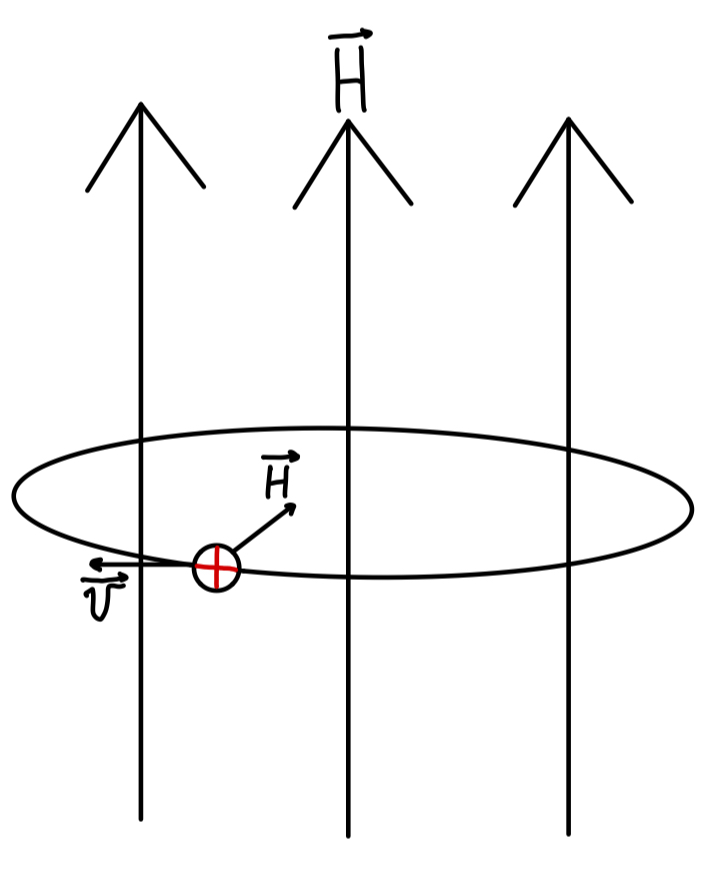
\includegraphics[width=\textwidth]{im/57.png}{\[\vec{v}\perp\vec{B} \]} % Ваше изображение
\end{minipage}%
\hfill
\begin{minipage}[c]{0.55\textwidth} % Правая часть: текст
    
    \[
    \vec{F}=\gamma m\dot{\vec{v}}=\frac{q}{c}[\vec{v}\times \vec{H}] \Rightarrow \dot{\vec{v}}=\left[ \left( -\frac{q\vec{H}}{\gamma mc}  \right) \times \vec{v} \right]
    \]
    \[
    \vec{\omega_c}=-\frac{q\vec{H}}{\gamma mc} 
    \]
\end{minipage}

\begin{figure}[h!]
    \centering
    % Первая картинка
    \begin{subfigure}{0.45\textwidth}
        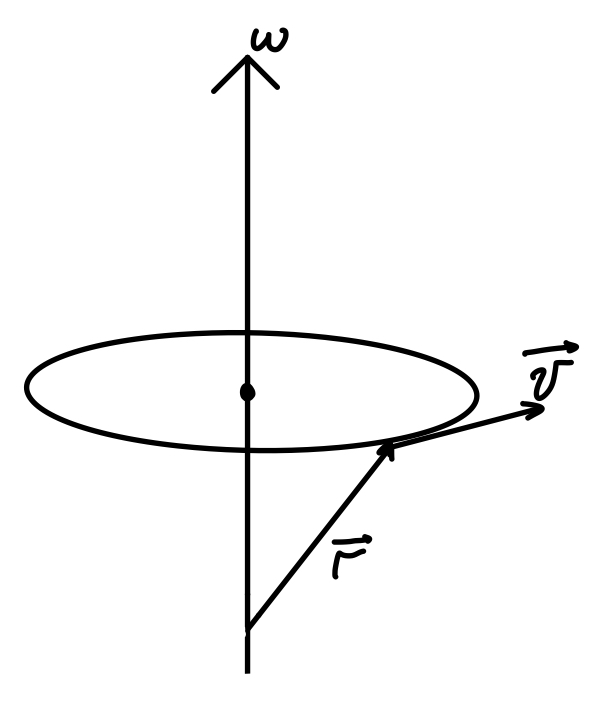
\includegraphics[width=\textwidth]{im/58.png} % Первая картинка
        \caption*{\(\vec{v}=\dot{\vec{r}}=[\vec{\omega}\times \vec{r}] \)}
        \label{fig:sub1}
    \end{subfigure}
    \hfill
    % Вторая картинка
    \begin{subfigure}{0.45\textwidth}
        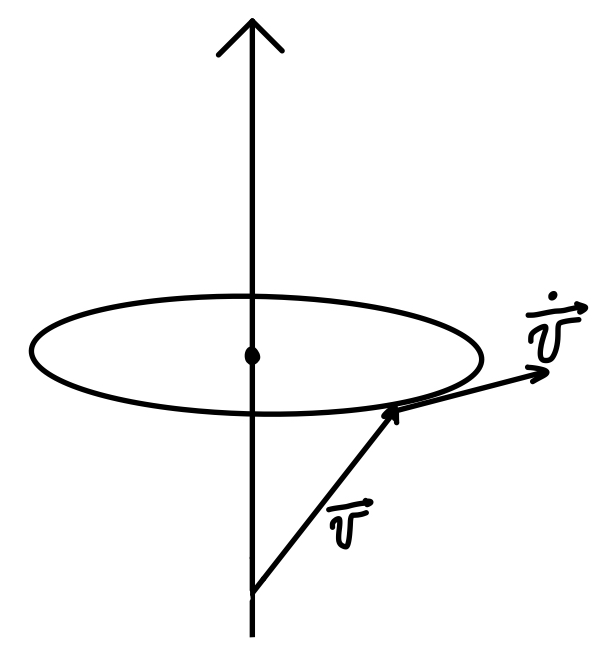
\includegraphics[width=\textwidth]{im/59.png} % Вторая картинка
        \caption*{\(\dot{\vec{v}}=[\vec{\omega_c}\times \vec{v}] \)}
        \label{fig:sub2}
    \end{subfigure}
    % Общая подпись для обеих картинок
    \caption*{}
    \label{fig:double}
\end{figure}

При малых скоростях:  $\omega_c= \frac{qH}{mc}.$

\[
\omega_c r=v_0 \Rightarrow r=\frac{v_0}{\omega_c} 
\]

\newpage

Неоднородное магнитное поле:

\imc[0.7\textwidth]{60.png}

В магнитном поле: $\vec{F}\perp\vec{v}\Rightarrow$ статичексое магнитное поле не совершает работу. 

\subsection*{Дрейф в скрещенных полях}

\imc[0.7\textwidth]{61.png}

\[
\vec{v}=\vec{\mathcal{U}}+\vec{\omega}
\]

Дрейфовая скорость, которая не зависит от $t -\vec{\omega}; $

Движение по окружнсоти + движение вдоль $\vec{H}$ с постоянной скоростью $ - \text{ }\vec{\mathcal{U} .}$

\[
m\dot{\vec{v}}=q\left( \vec{E}+\frac{q}{c}[\vec{v}\times \vec{H}]  \right)
\]

Пусть $\mathcal{U}$ есть решение уравнения без $\vec{E}: m\dot{\mathcal{U}}=\frac{q}{c}[\vec{v}\times\vec{H}]$

\[
\cancel{m\dot{\vec{\mathcal{U}}}}+m\dot{\vec{\omega}}=q\vec{E}+\cancel{\frac{q}{c}[\vec{\mathcal{U}}\times \vec{H}]}+\frac{q}{c}[\vec{\omega} \times \vec{H}] 
\]

Предпологаем, что $\vec{\omega}=\mathrm{const} \text{ и } \vec{\omega}\perp\vec{H}$, тогда $\dot{\vec{\omega}}=0:$

\[
q\vec{E}+\frac{q}{c}[\vec{\omega}\times \vec{H}]=0\Rightarrow[\vec{H}\times \vec{E}]+\frac{1}{c}[\vec{H}\times [\vec{\omega}\times \vec{H}]]=0  
\]

\[
c[\vec{H}\times \vec{E}]+\vec{\omega}H^2+H^2(\vec{\omega}\vec{H})=0\Rightarrow\boxed{\vec{\omega}=\frac{c[\vec{E}\times \vec{H}]}{H^2 }}\text{ } E<H
\]

Заряд движется вдоль эквипотенциали. 

\section*{28. Дивергенция магнитного поля. Вектор-потенциал. Кулоновская
калибровка.}
 
\subsection*{Дивергенция магнитного поля}

\noindent
\begin{minipage}[c]{0.2\textwidth} % Левая часть: изображение
    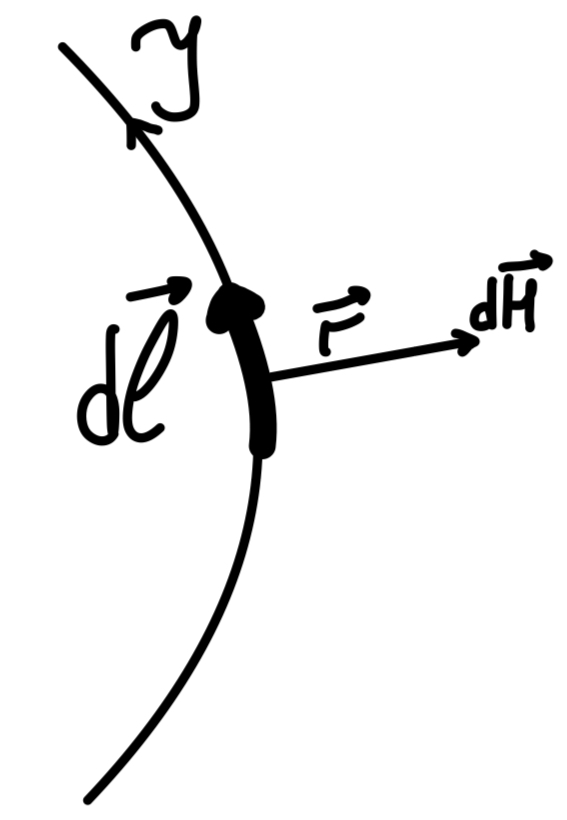
\includegraphics[width=\textwidth]{im/62.png}{} % Ваше изображение
\end{minipage}%
\hfill
\begin{minipage}[c]{0.68\textwidth} % Правая часть: текст
    
    \( d\vec{H}=\frac{I}{c}\left[ d\vec{l}\times \frac{\vec{r}}{r^3}  \right] \text{ Надо доказать, что: }\mathrm{div} \vec{H}=0 \)
    
    Принцип суперпозиции: $\vec{H}=\int d\vec{H}$
    
    Достаточно доказать, что $\mathrm{div} d\vec{H}$, так как $\mathrm{div}-$линеный оператор. 
\end{minipage}

\[
d\vec{H}=\frac{I}{c}\left[d\vec{l}\times \left( -\grad\left( \frac{1}{r}  \right) \right)\right] 
\]

Напомним: 

\[
\grad \left( \frac{1}{r}\right)=-\frac{1}{r^2}\grad(r)=\frac{1}{r^2}\frac{\vec{r}}{r} 
\]

\[
\mathrm{div}d\vec{H}=\frac{I}{c}\grad \left[ d\vec{l}\times \left( -\grad \left( \frac{1}{r}  \right) \right) \right]=\frac{I}{c}\left( d\vec{l} \underbrace{\left[ \grad \times \grad\left( \frac{1}{r}  \right) \right]}_{=0} \right) =0  
\]

\noindent
\begin{minipage}[c]{0.35\textwidth} % Левая часть: изображение
    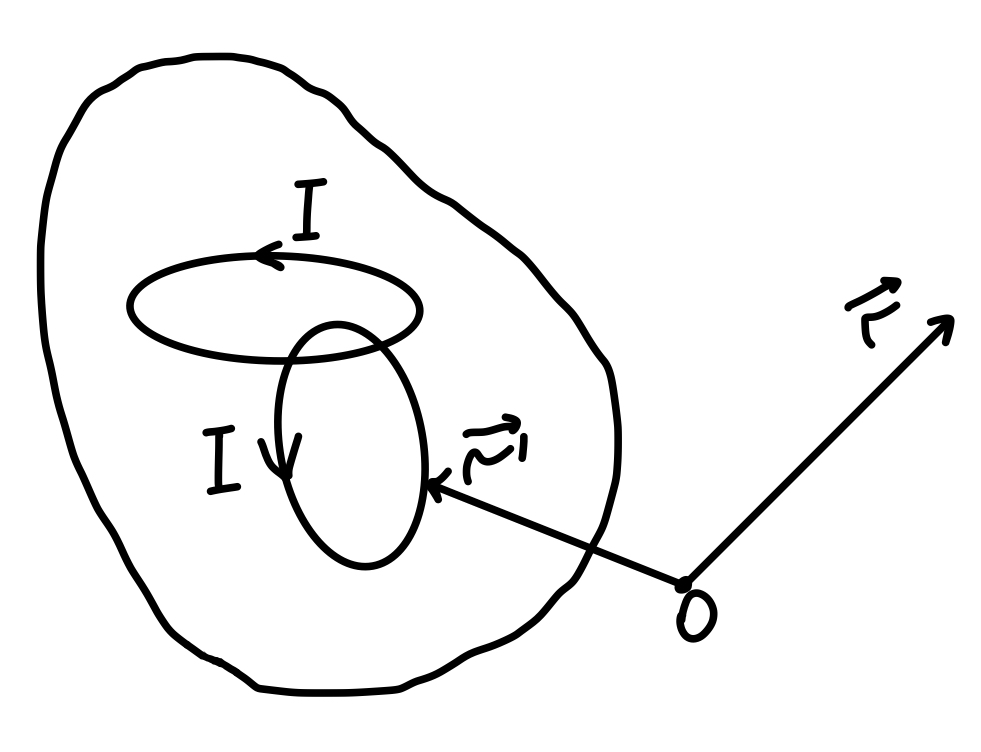
\includegraphics[width=\textwidth]{im/63.png}{} % Ваше изображение
\end{minipage}%
\hfill
\begin{minipage}[c]{0.7\textwidth} % Правая часть: текст
   
    \[
    \begin{array}{l|l}
        \vec{H}=\sum_{i} \frac{I_i}{c}\int \left[ d\vec{r'}\times \frac{\vec{r}-\vec{r'}}{|\vec{r}-\vec{r'}|^3}  \right] & \Rightarrow \\
        d\vec{l}\equiv d\vec{r'} & \\
        Id\vec{l}=\vec{j}dV' & \\
    \end{array}
    \]

\end{minipage}

\[
\begin{array}{|l}
    \Rightarrow \text{ т.о }\vec{H}=\underset{V}{\iiint}\frac{1}{c} \frac{[\vec{j}\times (\vec{r}-\vec{r'})]}{|\vec{r}-\vec{r'}|^3}dV' \\ 
    \vec{H}= \frac{1}{c} \underset{V}{\iiint} \left[ \vec{j}\times \left( -\frac{1}{|\vec{r}-\vec{r'}|} \right) \right]dV'
\end{array}
\]

Напомним: 

\[
\grad:=\frac{\partial}{\partial \vec{r}}; \grad ' := \frac{\partial}{\partial \vec{r'}}
\]

\[
\mathrm{div}\vec{H}=\frac{1}{c}\underset{V}{\iiint}\left( \grad \left[ \vec{j} \times \grad \left( -\frac{q}{|\vec{r}-\vec{r'}|}  \right) \right] \right)dV'= \frac{1}{c}\underset{V}{\iiint}\left( \vec{j}\underbrace{\left[ \grad \times \grad \frac{1}{|\vec{r}-\vec{r'}|}  \right]}_{=0} \right)dV'
\]

\subsection*{Вектор-потенциал}

$\mathrm{div}\vec{H}=0\Rightarrow \vec{H} $ можно подставить в виде $\mathrm{rot} $ некоторого вектора.

\[
\vec{H}\overset{df}{=}\mathrm{rot}\vec{A} 
\]

Определить вектор поля одним только $\mathrm{rot} $ нельзя. 

\[
\begin{aligned}
    \begin{array}{l|l}
        \begin{cases}
            \mathrm{div}\vec{A_1}=\mathrm{div}\vec{A_2} \qquad \vec{A}=\vec{A_1}-\vec{A_2} \\
            \mathrm{rot}\vec{A_1}=\mathrm{rot}\vec{A_2}    
        \end{cases}   
    \end{array}
    \Rightarrow
    \begin{cases}
        \mathrm{div}\vec{A}=0 \\
        \mathrm{rot}\vec{A}=0 \Rightarrow \vec{A}=-\grad\varphi 
    \end{cases}
\end{aligned}
\]

\[
\begin{cases}
    \vec{A}=\grad\varphi \\
    \Delta\varphi=0
\end{cases}
\]

Можно взять $\vec{A}=\frac{1}{c}\underset{V}{\iiint} \frac{\vec{j}(\vec{r'})}{|\vec{r}-\vec{r'}|}dV'$( где $V$ предыдущий объём)

Покажем, что $\mathrm{rot}\vec{A}=\vec{H} \text{ и } \mathrm{div}\vec{A}=0: $

\[
\mathrm{rot}\vec{A}=\frac{1}{c}\underset{V}{\iiint} \left[ \grad \times \frac{\vec{j}(\vec{r'})}{|\vec{r}-\vec{r'}|}  \right]dV'=\frac{1}{c}\iiint \left[ \vec{j}\times \left( -\frac{1}{|\vec{r}-\vec{r'}|}  \right) \right] dV'=\vec{H} \quad \blacksquare
\]

\[
\mathrm{div}\vec{A}=\frac{1}{c}\underset{V}{\iiint}\grad \vec{j}\frac{1}{|\vec{r}-\vec{r'}|}dV'=\frac{1}{c}\underset{V}{\iiint} \vec{j}\grad \frac{1}{|\vec{r}-\vec{r'}|}dV'\fbox{=}
\]

Уточнение:

\[
\grad \frac{1}{|\vec{r}-\vec{r'}|}=-\grad ' \frac{1}{|\vec{r}-\vec{r'}|}  
\]
 
\[
\fbox{=}-\frac{1}{c}\underset{V}{\iiint}\vec{j}(\vec{r'})\grad ' \overset{\downarrow}{\frac{1}{{|\vec{r}-\vec{r'}|}}}dV'=-\frac{1}{c}\underset{V}{\iiint}\overset{\downarrow}{\vec{j}}(\vec{r'})\grad ' \overset{\downarrow}{\frac{1}{|\vec{r}-\vec{r'}|} }dV'+
\]

\[
    +\frac{1}{c}\underset{V}{\iiint}\overset{\downarrow}{\vec{j}}(\vec{r'})\grad ' \frac{1}{{|\vec{r}-\vec{r'}|}}dV'\fbox{=}
\]

\newpage

\[
\fbox{=}-\frac{1}{c}\underset{V}{\iiint} \mathrm{div} \left( \frac{\vec{j}(\vec{r'})}{|\vec{r}-\vec{r'}|} \right) dV'+\frac{1}{c}\underset{V}{\iiint}\frac{1}{|\vec{r}-\vec{r'}|}\mathrm{div}(\cancelto{0}{\vec{j}(\vec{r'})})dV'\fbox{=}
\]

\[
\fbox{=}\underbrace{-\frac{1}{c}\underset{\delta V}{\oiint} \frac{\cancelto{0}{\vec{j}(\vec{r'})}}{|\vec{r}-\vec{r'}|}dS'}_{\text{на границе нет токов}}+\underbrace{0}_{\text{по З.С.З}}=0 \quad \blacksquare
\]

Закон сохранения заряда:

\[
\frac{\partial \rho}{\partial t} +\mathrm{div}\vec{j}=0 \text{, стационарный случай } \left( \frac{\partial \rho}{\partial t}  \right)=0 \Rightarrow \mathrm{div}\vec{j}=0  
\]

\textit{Ротор магнитного тока:}

\[
(\overset{a}{\grad}\times[\overset{b}{\grad}\times \overset{c}{\vec{A}}])\overset{bac-cab}{=}\grad\cdot[\grad\cdot\vec{A}]-(\grad\cdot\grad)\cdot\vec{A}
\]

Вспомним $\mathrm{rot}(\mathrm{rot}\vec{A})=\mathrm{grad}(\mathrm{div}\vec{A})-\Delta \vec{A}$

\[
\begin{aligned}
    \begin{array}{l|l}
        \vec{H}=\mathrm{rot}\vec{A}, \\ 
        \text{где }\vec{A}=\frac{1}{c}\underset{V}{\iiint}\frac{\vec{j}(\vec{r'})}{|\vec{r}-\vec{r'}|}  
    \end{array}
    \Rightarrow \mathrm{rot}\vec{H}=  \mathrm{rot}(\mathrm{rot}\vec{A} )= \mathrm{grad}(\cancelto{0}{\mathrm{div}\vec{A} })-\Delta\vec{A} \fbox{=} \\
\end{aligned}
\]

\[
\fbox{=}\frac{1}{c}\underset{V}{\iiint}\vec{j}(\vec{r'})\Delta \frac{1}{|\vec{r}-\vec{r'}|}dV'=\frac{1}{c}\underset{V}{\iiint}\vec{j}(\vec{r'})4\pi\delta(\vec{r}-\vec{r'})dV' = 
\]

\[
=\frac{4\pi}{c}\underset{V}{\iiint}\vec{j}(\vec{r'})\delta (\vec{r}-\vec{r'})dV'=\frac{4\pi}{c}\vec{j}(\vec{r})  
\]

\[
\text{Итог: } \boxed{\mathrm{rot}\vec{H}=\frac{4\pi}{c}\vec{j}  }
\]
    \newpage
\section{Скалярный потенциал магнитного поля.}
 
Согласно первому уравнению Максвелла в тех местах, где есть плотность тока, ротор вектора напряженности не равен нулю и поле имеет вихревой характер. В тех областях, где плотность тока равна нулю ($\delta =0$) $\mathrm{rot}\vec{H}$  , магнитное поле можно рассматривать как потенциальное



\noindent
\begin{minipage}[c]{0.3\textwidth} % Левая часть: изображение
    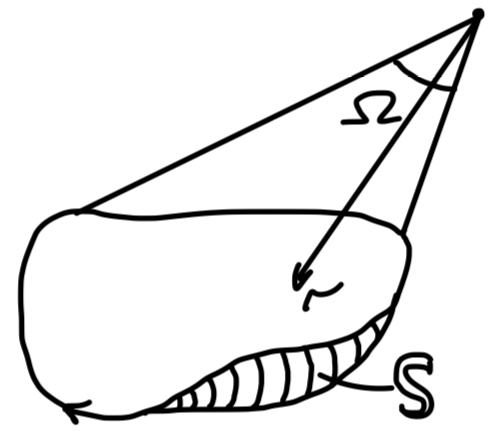
\includegraphics[width=\textwidth]{im/64.png}{} % Ваше изображение
\end{minipage}%
\hfill
\begin{minipage}[c]{0.55\textwidth} % Правая часть: текст
    \( \mathrm{rot}\vec{H}=\frac{4\pi}{c}\vec{j}   \) 
    
    \( \psi: \vec{H}=-\grad \psi \)
    
    \( \psi = \frac{I}{c}\Omega  \) 

    \( \Omega =\underset{S}{\iint}\frac{d\vec{S}}{r^2} \frac{\vec{r}}{r}   \) 
\end{minipage}
\[\text{ }\]
\noindent
\begin{minipage}[c]{0.4\textwidth} % Левая часть: изображение
    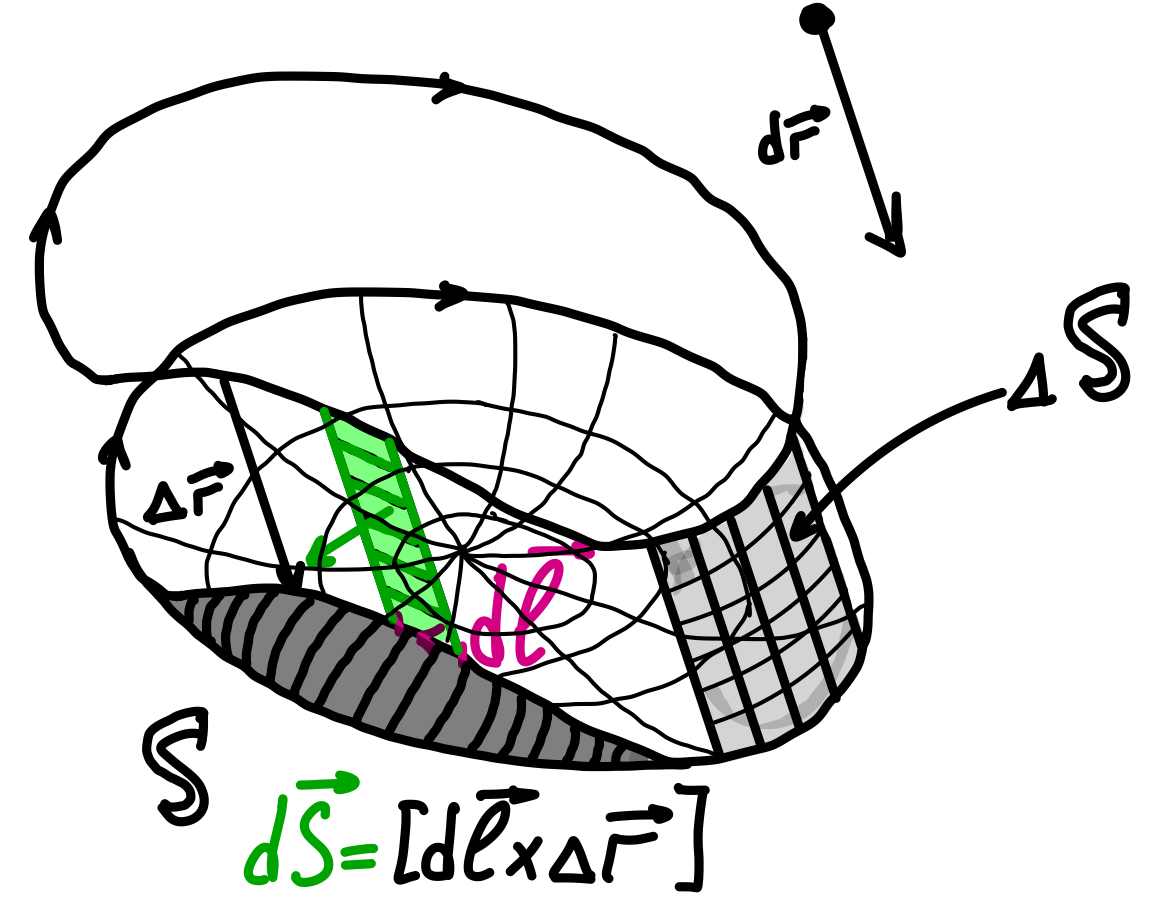
\includegraphics[width=\textwidth]{im/65.png}{} % Ваше изображение
\end{minipage}%
\hfill
\begin{minipage}[c]{0.55\textwidth} % Правая часть: текст
    \( \Delta\Omega =(\grad\Omega)\Delta \vec{r} \) 

    \( \Omega= \underset{S}{\iint}\frac{\vec{r}}{r^3}d\vec{S};\quad \Omega+\Delta\Omega =\underset{S+\Delta S}{\iint} \frac{\vec{r}}{r^3}d\vec{S};  \)
    
    \( \Delta\Omega= \underset{\Delta S}{\iint} \frac{\vec{r}}{r^3}dS= \oint \left( \frac{\vec{r}}{r^3}[d\vec{l}\times \Delta\vec{r}]  \right)=  \)

    \(\qquad = \Delta\vec{r} \oint \left[ \frac{\vec{r}}{r^3}\times d\vec{l}  \right] \Rightarrow   \) 
\end{minipage}

\[
\Rightarrow \grad\Omega=\oint \left[ \frac{\vec{r}}{r^3}\times d\vec{l}  \right]
\]

\[
\vec{H}=\frac{I}{c}\oint \left[ \frac{d\vec{l} \times \vec{r}}{r^3}  \right] = -\frac{I}{c} \grad \psi
\]
    \newpage
\section*{30. Поток и циркуляция магнитного поля. Дифференциальная и интегральная
форма уравнений магнитостатики. Граничные условия.}

\subsection*{Поток и циркуляция магнитного поля и Дифференциальная и интегральная
форма уравнений магнитостатики}

\begin{center}
    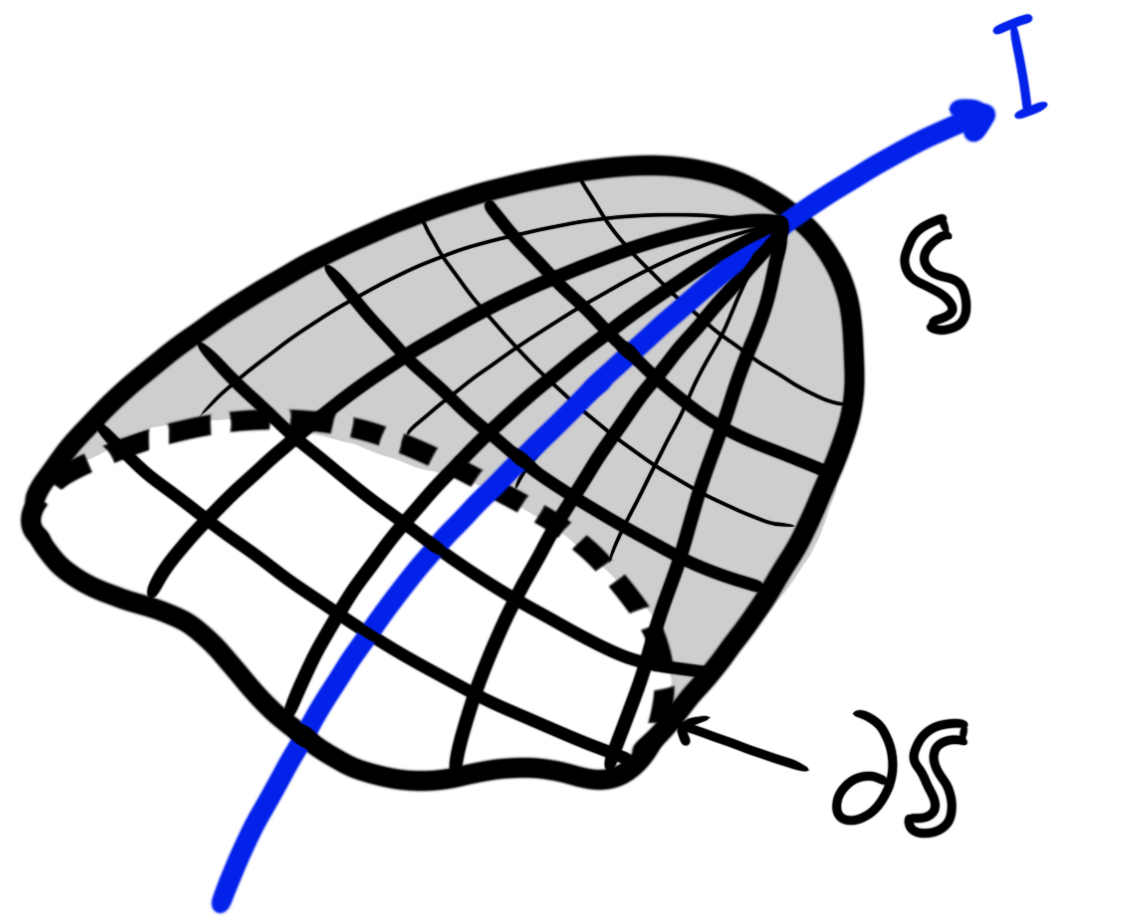
\includegraphics[width=0.5\textwidth]{im/66.png}
\end{center}

Где $I$ - полный ток через поверхность $S$. 
 
\begin{gather*}
    \mathrm{rot}\vec{H}=\frac{4\pi}{c}\vec{j}\Rightarrow \underset{S}{\iint}\mathrm{rot}\vec{H}\cdot d\vec{S}=\frac{4\pi}{c}\iint \vec{j}\cdot d\vec{S}  \\
    \Downarrow \\
    \boxed{\underset{\delta S}{\oint}\vec{H}d\vec{l}=\frac{4\pi}{c}I }\textit{ - циркуляция}
\end{gather*}

\begin{gather*}
    \mathrm{div}\vec{H}=0\Rightarrow \ \underset{V}{\iiint}\mathrm{div}\vec{H}dV=0=\underset{\delta V}{\oiint}\vec{H}d\vec{S}(\text{так как}\forall V) \\
    \Downarrow \\
    \boxed{\oiint \vec{H}d\vec{S}=0}\textit{ - поток}
\end{gather*}

\newpage

\subsection*{Граничные условия}

\begin{minipage}[c]{0.5\textwidth} % Левая часть: изображение
    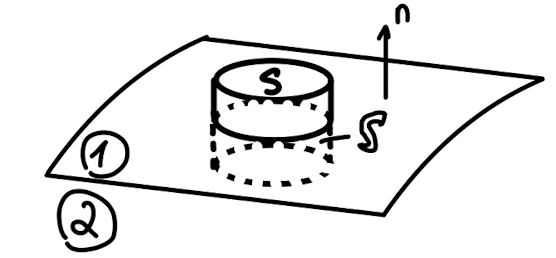
\includegraphics[width=\textwidth]{im/67.png} % Ваше изображение
\end{minipage}%
\hfill
\begin{minipage}[c]{0.55\textwidth} % Правая часть: текст
    \begin{gather*}
        \oiint \vec{H}d\vec{S}=0 \\
        H_{1n}|\cdot S-H_{2n}|\cdot S=0 \\
        \Downarrow \\
        \boxed{H_{1n}=H_{2n}} \text{ - то есть } H_n \text{ - непр.}
    \end{gather*}
\end{minipage}
\( \text{ } \)  
\begin{minipage}[c]{0.5\textwidth} % Левая часть: изображение
    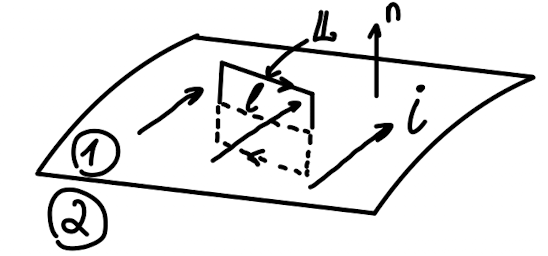
\includegraphics[width=\textwidth]{im/68.png} % Ваше изображение
\end{minipage}%
\hfill
\begin{minipage}[c]{0.55\textwidth} % Правая часть: текст
    \begin{gather*}
        \underset{L}{\oint}\vec{H}d\vec{l}=\frac{4\pi}{c}I \\
        H_{1\tau}\cdot l - H_{2\tau}\cdot l =\frac{4\pi}{c}il \\
        \Downarrow \\
        \boxed{H_{1\tau}- H_{2\tau} = \frac{4\pi}{c}i }
    \end{gather*}
\end{minipage}




\section*{31. Основное уравнение магнитостатики и его общее решение для
безграничного пространства. Магнитный диполь. Вектор-потенциал и
магнитное поле диполя.}
 
\subsection*{Основное уравнение магнитостатики и его общее решение для
безграничного пространства}

Воспользуемся уравнением магнитостатики:

\[
\mathrm{rot}\vec{H}=\frac{4\pi}{c}\vec{j}  
\]

и подставим его в:

\[
\vec{H}=\mathrm{rot}\vec{A}
\]

Получим:
\[
\mathrm{rot}(\mathrm{rot}\vec{A} )=\frac{4\pi}{c}\vec{j}  
\]

Двойной ротор в левой части уравнения преобразуем, используя известную формулу векторного анализа:

\[
\mathrm{rot}(\mathrm{rot}\vec{A} )=-\Delta \vec{A}+ \grad \mathrm{div}\vec{A} 
\]

и используем кулоновскую калибровку потенциала:

\[
\mathrm{div}\vec{A}=0 
\]

В результате получим \textit {основное уравнение} магнитостатики:

\[
\boxed{\Delta \vec{A}=-\frac{4\pi}{c}\vec{j} }
\]

По аналогии с уравнением Пуассона $\Delta\varphi=-4\pi\rho$ и его общим решением $\varphi(\vec{r})=\int \frac{\rho(\vec{r'}dV')}{|\vec{r}-\vec{r'}|}=\frac{q}{|\vec{r}-\vec{r'}|}$ нетрудно догадаться, что общее решение уравнения можно записать следующим образом:

\[
\boxed{\vec{A}=\frac{1}{c}\int \frac{\vec{j}(\vec{r'})dV'}{|\vec{r}-\vec{r'}|}  }
\]

\subsection*{Магнитный диполь и Вектор-потенциал и
Магнитное поле диполя}

\begin{center}
    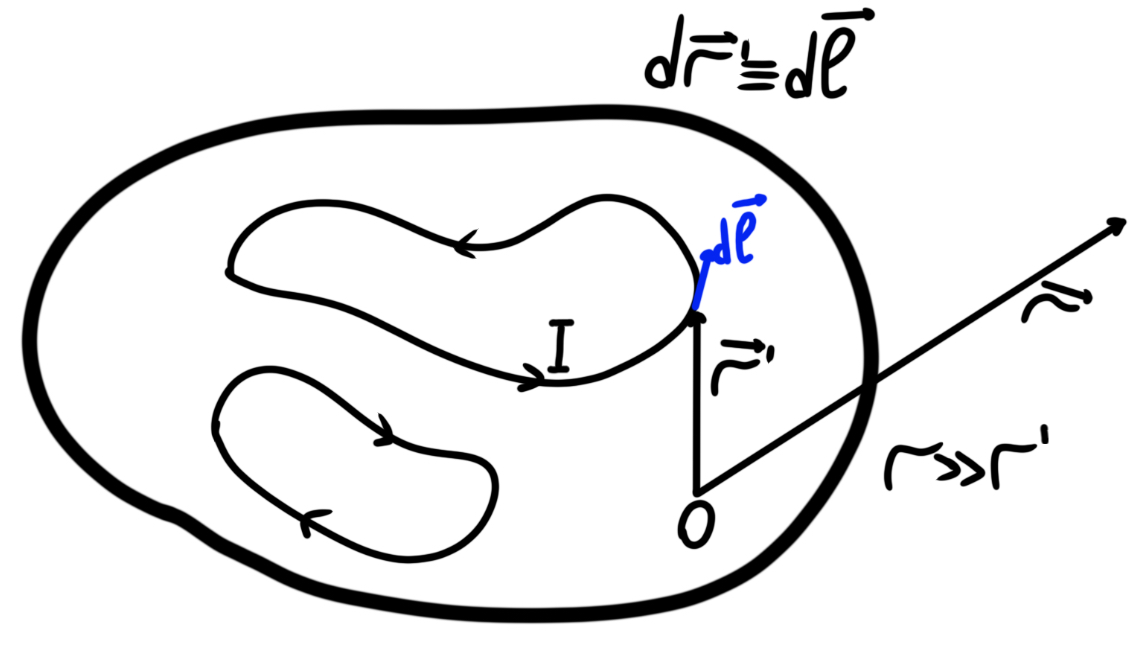
\includegraphics[width=0.5\textwidth]{im/69.png}
\end{center}

\begin{gather*}
    \vec{A}=\frac{q}{c} \iiint \frac{\vec{j}(\vec{r'})}{|\vec{r}-\vec{r'}|}dV'=\sum \frac{I}{c}\oint \frac{1}{|\vec{r}-\vec{r'}|}d\vec{r'} \\
    \text{в дальнейших формулах не будем писать }\Sigma \\
    \vec{j}dV'\rightarrow Id\vec{l}=Id\vec{r'} 
\end{gather*}

Вспомним разложение:

\[
\frac{1}{|\vec{r}-\vec{r'}|} =\frac{1}{r}+\frac{\vec{r}\cdot\vec{r'}}{r^3}+\dots (\text{ограничемся двумя членами})
\]

\begin{gather*}
    \vec{A}
\end{gather*}
    \newpage
\section{Сила и момент сил, действующие на магнитный диполь в
слабонеоднородном магнитном поле.}

\textit{Момент сил действующий на магнитный диполь в однородном поле:}

\begin{gather*}
    \vec{m}=\frac{I}{2c} \oint [\vec{r'}\times d \vec{r'}] \\
    \vec{M}=\oint \left[ \vec{r}\times \frac{I}{c} [d\vec{r}\times \vec{H}]  \right]=\frac{I}{c}\oint [\vec{r}\times [d\vec{r}\times \vec{H}]]= \\
    =\frac{I}{c}\oint (\vec{r}\vec{H})d\vec{r} -\frac{I}{c}\vec{H} \cancelto{0}{\oint \vec{r}d\vec{r}}=\frac{I}{c} \cancelto{0}{(\vec{r}\vec{H})}\vec{r}|-\frac{I}{c}\oint \vec{r}(\vec{H}d\vec{r})= \\
    =\frac{I}{2c}\oint \left( \overset{b}{d\vec{r}}(\overset{a}{\vec{H}}\overset{c}{\vec{r}})-\overset{c}{\vec{r}}(\overset{a}{\vec{H}}\overset{b}{d\vec{r}}) \right)=\frac{I}{2c}\oint[\vec{H}\times [d\vec{r}\times \vec{r}]]= \\
    =\left[ \frac{I}{2c}\oint[\vec{r}\times d\vec{r}]\times \vec{H}  \right]=[\vec{m}\times \vec{H}]     
\end{gather*}

\[
\boxed{\vec{M}=[\vec{m}\times \vec{H}]}
\]

\textit{Сила в однородном поле:}

\[
\vec{F}=\frac{I}{c}\oint [d\vec{r}\times \vec{H}]=\frac{I}{c} \left[ \oint \cancelto{0}{d\vec{r}}\times \vec{H} \right] =0
\]

\textit{Сила в слабонеоднородном поле:}

\begin{minipage}[c]{0.25\textwidth} % Левая часть: изображение
    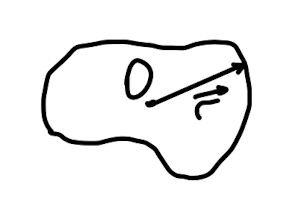
\includegraphics[width=\textwidth]{im/71.png} % Ваше изображение
\end{minipage}%
\hfill
\begin{minipage}[c]{0.55\textwidth} % Правая часть: текст
    \( \vec{H}=\vec{H_0}+(\vec{r}\gradd)\vec{H} \) 
\end{minipage}

\begin{gather*}
    \vec{F}=\frac{I}{c}\oint [d\vec{r}\times (\vec{r}\gradd)\vec{H}]=\frac{I}{c}\left[ \oint d\vec{r}(\vec{r}\gradd)\times \vec{H} \right]  \fbox{=}\\
    \oint d\vec{r}(\vec{r}\gradd)=\vec{r} \cancelto{0}{(\vec{r}\gradd)}| - \oint \vec{r}(d\vec{r}\gradd)=\frac{1}{2} \left[ d\vec{r}(\gradd\vec{r})-\vec{r}(d\vec{r}\gradd) \right]= \\
    =\frac{1}{2}\oint [\gradd \times [d\vec{r}\times \vec{r}]]  \\
    \text{Тогда:} \frac{I}{c}\oint d\vec{r}(\vec{r}\gradd)=\frac{I}{2c}\oint [[\vec{r}\times d\vec{r}]\times \gradd]=[\vec{m}\times \grad]  \\ 
    \fbox{=}[[\vec{m}\times \grad]\times \vec{H}]=[\overset{\downarrow}{\vec{H}}\times [\grad \times \vec{m}]]= \grad(\vec{H}\vec{m})-\vec{m}\cancelto{0}{\grad\vec{H}}
\end{gather*}

\[
\boxed{\vec{F}=\grad(\vec{H}\vec{m})}
\]

    \newpage
\section*{33. Магнитное поле в среде. Молекулярные токи. Вектор намагниченности,
его связь с молекулярными токами.}
    \newpage
\section{Векторы В и Н. Магнитная проницаемость. Полная система уравнений для
магнитного поля в среде.}

\subsection*{Векторы В и Н}

\[
\begin{aligned}
    \begin{cases}
        \mathrm{div}\vec{H}=0  \\ 
        \mathrm{rot}\vec{H}=\frac{4\pi}{c}(\vec{j}+\vec{j}_{\text{м}})
    \end{cases}
    \overset{\text{уср}}{\rightarrow}
    \begin{cases}
        \quad \mathrm{div}<\vec{H}>=0 \\
        \mathrm{rot}<\vec{H}= \frac{4\pi}{c}(\vec{j}+<\vec{j}_{\text{м}}>)
    \end{cases}
    \rightarrow
\end{aligned}
\]

\[
\begin{aligned}
    \overset{<\vec{H}>=:\vec{B}}{\rightarrow}
    \begin{cases}
        \mathrm{div}\vec{B}=0 \\
        \mathrm{rot}\vec{B}= \frac{4\pi}{c}(\vec{j}+<\vec{j}_{\text{м}}>)
    \end{cases}
    \overset{<\vec{j}_{\text{м}}>=c\cdot \mathrm{rot}\vec{M}}{\rightarrow}
    \begin{cases}
        \mathrm{div}\vec{B}=0 \\
        \mathrm{rot}(\vec{B}-4\pi\vec{M})= \frac{4\pi}{c}\vec{j}
    \end{cases}
    \rightarrow 
\end{aligned}
\]

\[
\begin{aligned}
    \overset{\vec{B}-4\pi\vec{M}=:\vec{H}}{\rightarrow}
    \boxed{\begin{cases}
        \mathrm{div}\vec{B}=0 \\
        \mathrm{rot}\vec{H}= \frac{4\pi}{c}\vec{j}
    \end{cases}
    }
\end{aligned}
\]

\[
\vec{B}=(1-4\pi\chi)\vec{H}
\]

\[
\text{(Рекумендуется просмотр прошлого вопроса для полноты ответа) }
\]

\subsection*{Магнитная проницаемость}

\[
\mu=1+4\pi\chi
\]

\subsection*{Полная система уравнений для
магнитного поля в среде}

\[
    \begin{cases}
        \mathrm{div}\vec{B}=0 \\
        \mathrm{rot}\vec{H}= \frac{4\pi}{c}\vec{j}
    \end{cases}
\]
 

    \newpage
\section*{35. Интегральный вид уравнений Максвелла и граничные условия для
магнитного поля при наличии сред.}

\begin{minipage}[c]{0.4\textwidth} % Левая часть: изображение
    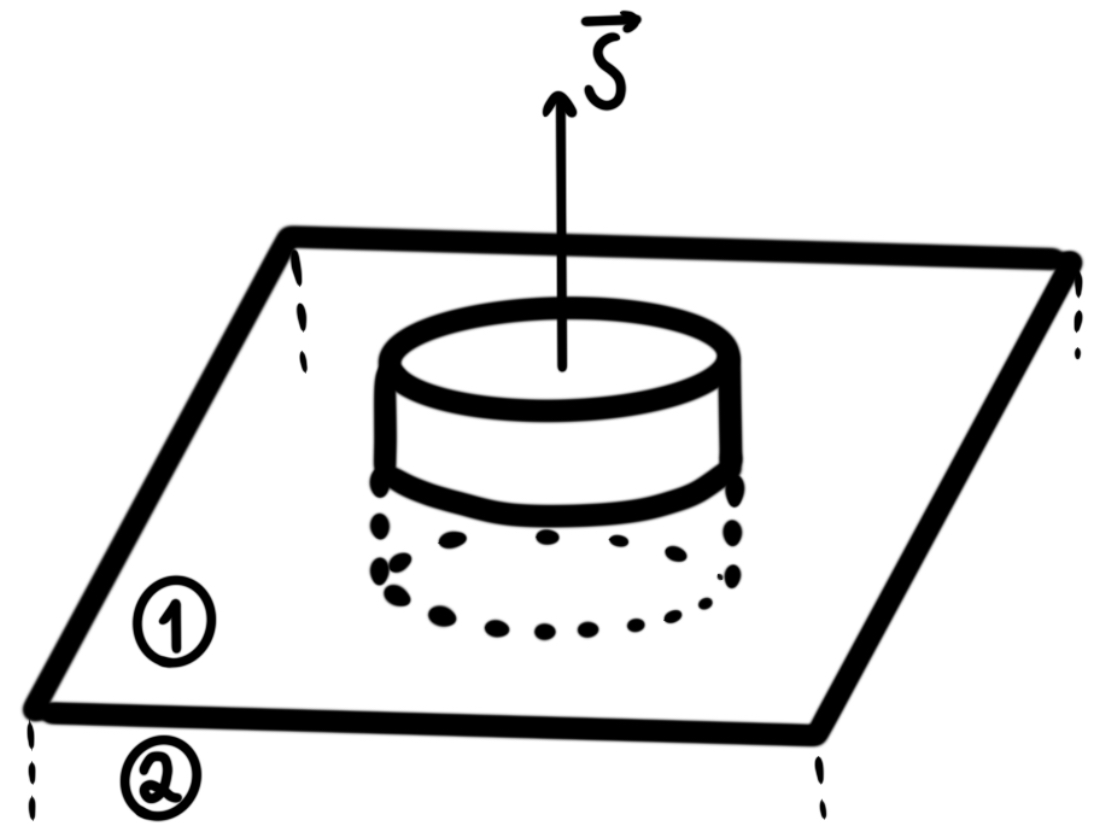
\includegraphics[width=\textwidth]{im/73.png} % Ваше изображение
\end{minipage}%
\hfill
\begin{minipage}[c]{0.7\textwidth} % Правая часть: текст
    \begin{gather*}
        \mathrm{div}\vec{B}=0 \\
        \downarrow \\
        \oiint \vec{B}d\vec{S}=0 
    \end{gather*}
\end{minipage}

\[
B_{1n}|\cdot S-B_{2n}|\cdot S=0 \Rightarrow \boxed{B_n|-\text{непр.}}
\]

\begin{minipage}[c]{0.4\textwidth} % Левая часть: изображение
    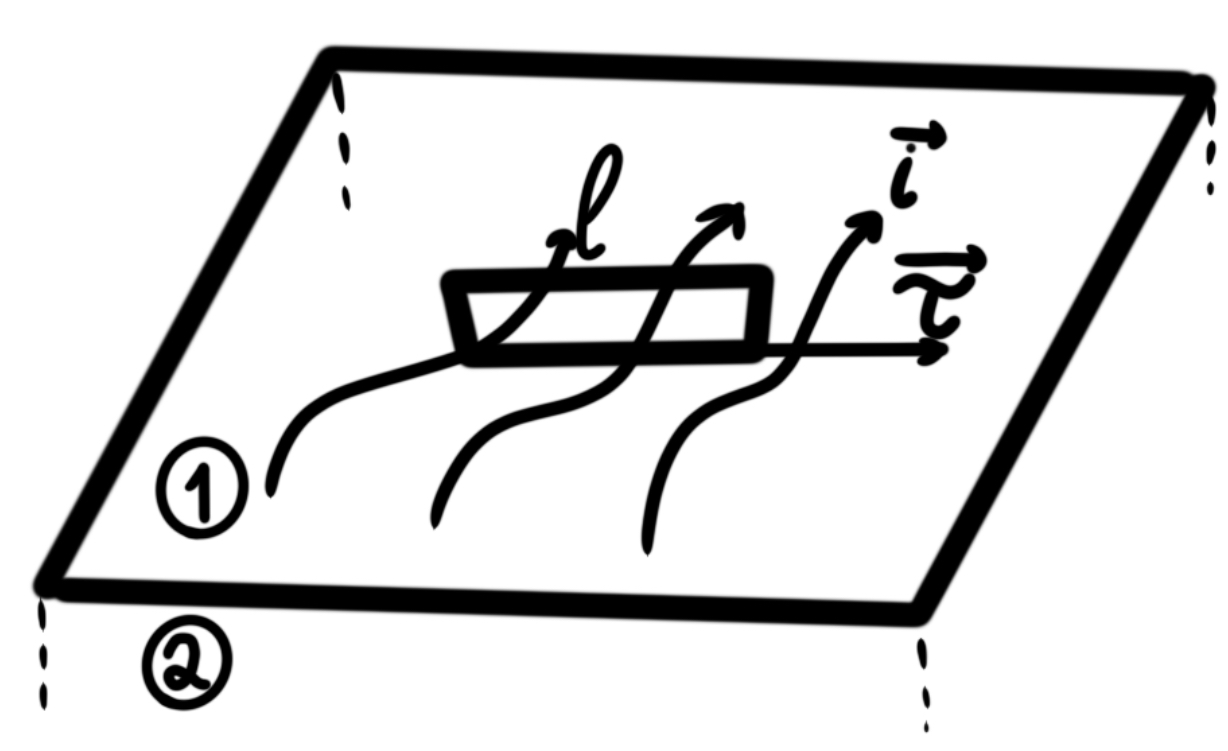
\includegraphics[width=\textwidth]{im/74.png} % Ваше изображение
\end{minipage}%
\hfill
\begin{minipage}[c]{0.6\textwidth} % Правая часть: текст
    \begin{gather*}
        \mathrm{rot}\vec{H}=\frac{4\pi}{c}\vec{j}  \\
        \downarrow \\
        \oint \vec{H}d\vec{l}=\frac{4\pi}{c} 
    \end{gather*}
\end{minipage}

\[
H_{1\tau}|\cdot l -H_{2\tau}|\cdot l=\frac{4\pi}{c}il \Rightarrow \boxed{H_{1\tau}|-H_{2\tau}|=\frac{4\pi}{c}i } 
\]

\section{Диамагнетики. Гиромагнитное отношение. Ларморовская прецессия.
Оценка магнитной проницаемости.}

\subsection*{Диамагнетики}

\[
1)\chi<0;\qquad2)|\chi|<<1;
\]

\[
\grad(\vec{m}\vec{H})=\grad(-|\chi|H^2)=-|\chi|\grad H^2
\]

\subsection*{Гиромагнитное отношение}

\begin{minipage}[c]{0.4\textwidth} % Левая часть: изображение
    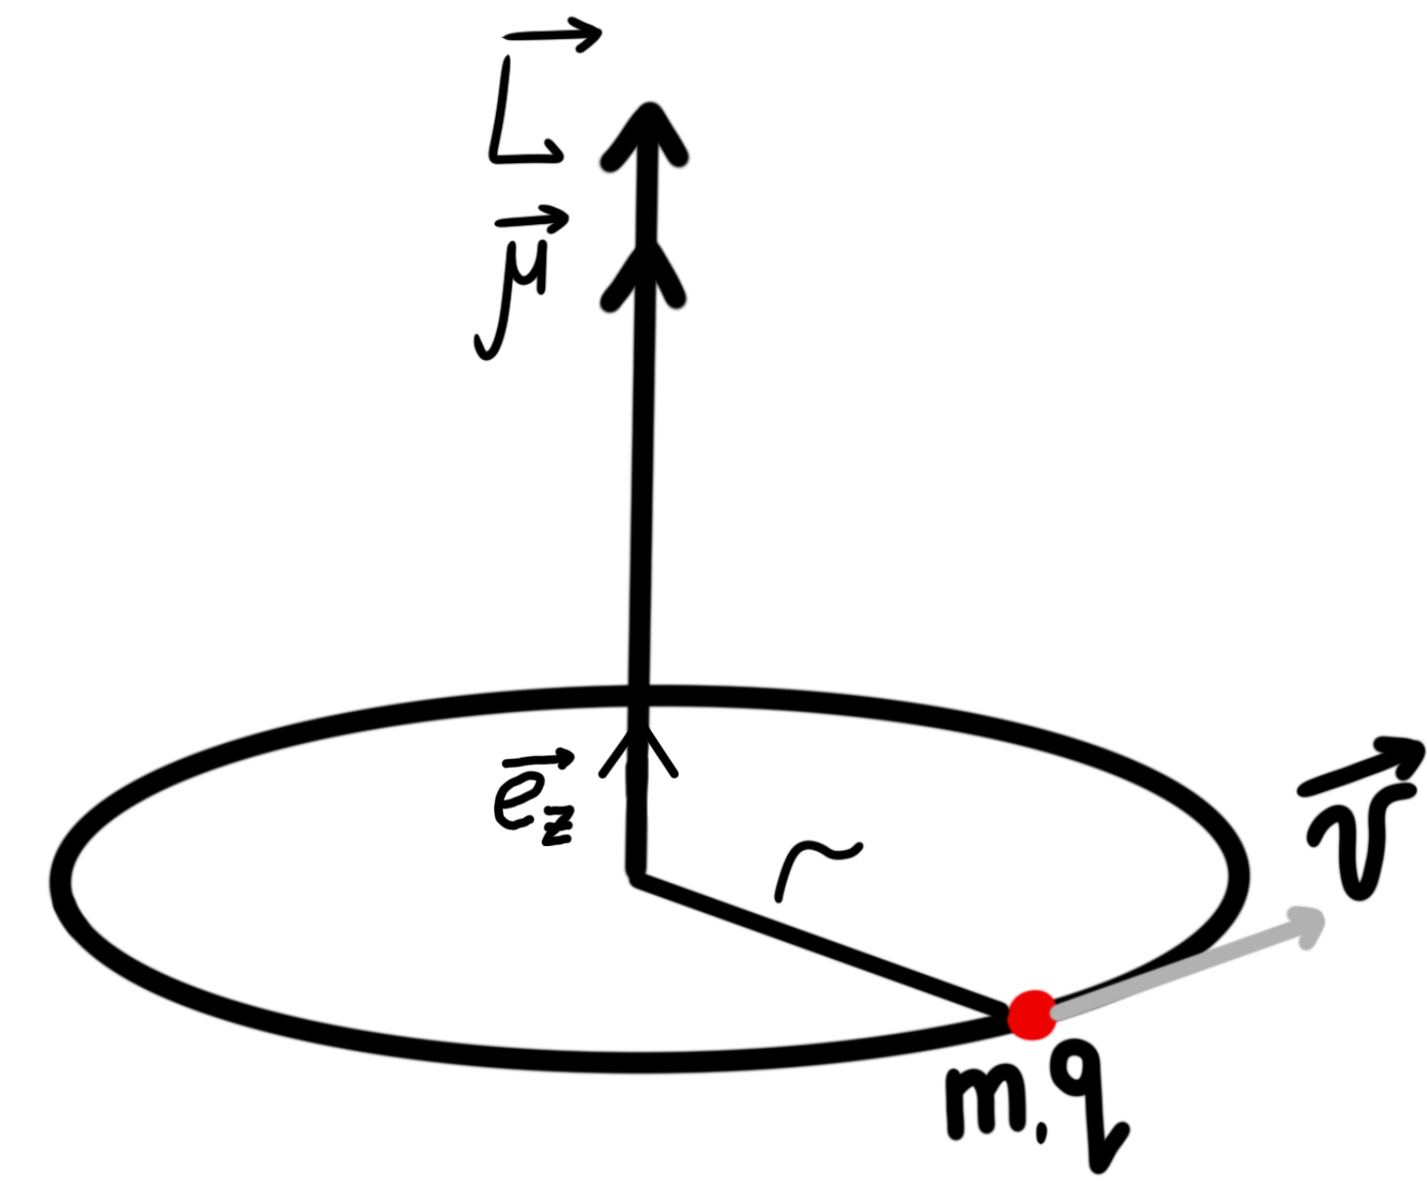
\includegraphics[width=\textwidth]{im/75.png} % Ваше изображение
\end{minipage}%
\hfill
\begin{minipage}[c]{0.6\textwidth} % Правая часть: текст
    \[
    \begin{array}{l|l}
        \vec{\mu}= \frac{I}{c}\vec{S}=\frac{q}{cT}\vec{S}=\frac{q}{cT}\pi r^2 \vec{e_z} & \Rightarrow \\
        \vec{L}=mr\vec{e_z}=\frac{2\pi mr^2}{T}\vec{e_z} 
    \end{array}
    \]
    \[
    \Rightarrow \vec{\mu}=\eta  \vec{L}, \text{ где } \eta=\frac{q}{2mc} 
    \]
    \[
    \eta\text{- гиромагнитное отношение}
    \]
\end{minipage}

\subsection*{Ларморовская прецессия}

\begin{minipage}[c]{0.2\textwidth} % Левая часть: изображение
    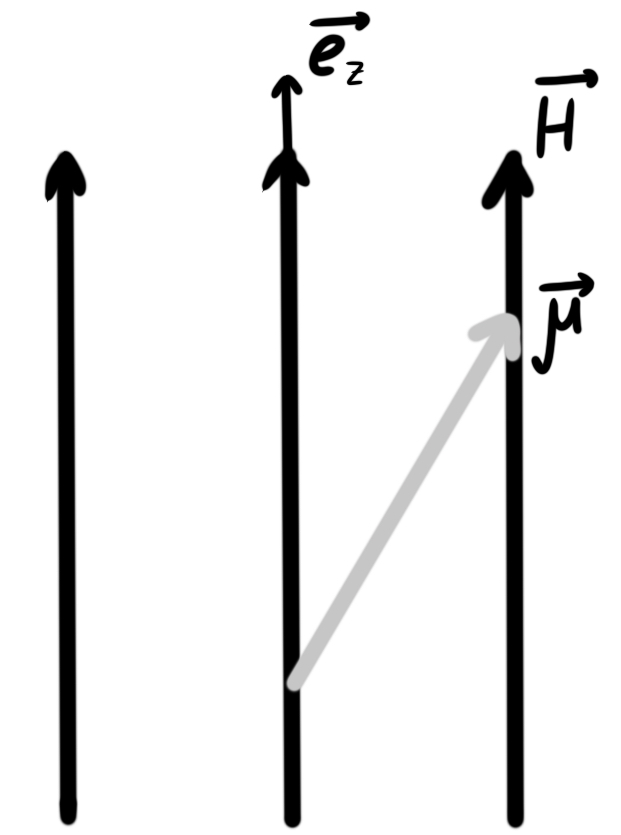
\includegraphics[width=\textwidth]{im/76.png} % Ваше изображение
\end{minipage}%
\hfill
\begin{minipage}[c]{0.6\textwidth} % Правая часть: текст
    \[
    \begin{aligned}
        \frac{d\vec{L}}{dt}=\overset{\text{момент сил}}{\vec{M}}=[\vec{\mu}\times \vec{H}]=[\eta\vec{\nu}\times \vec{H}]=[-\eta\vec{H}\times \vec{L}] \\
        \frac{d\vec{L}}{dt}=[-\eta\vec{H}\times \vec{L}]
    \end{aligned}
    \]
\end{minipage}

\begin{minipage}[c]{0.5\textwidth} % Левая часть: изображение
    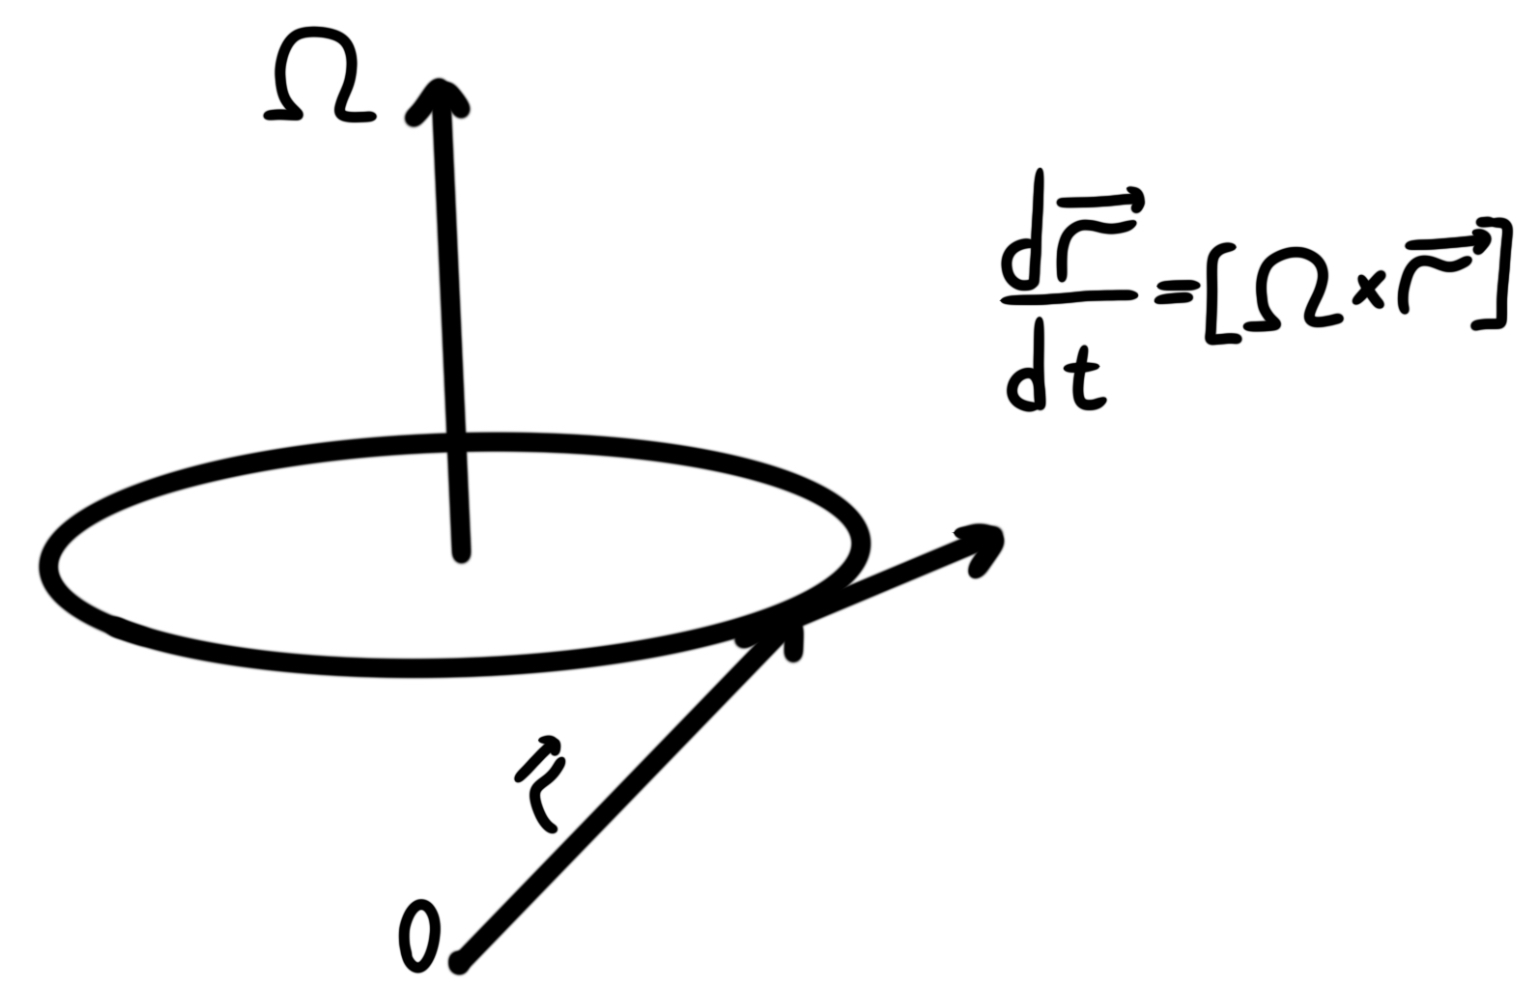
\includegraphics[width=\textwidth]{im/77.png} % Ваше изображение
\end{minipage}%
\hfill
\begin{minipage}[c]{0.6\textwidth} % Правая часть: текст
    \[
     \frac{d\vec{L}}{dt}=[-\eta\vec{H}\times \vec{L}]\Rightarrow\vec{\Omega_{\text{л}}}=-\eta\vec{H}
    \]
\end{minipage}

\subsection*{Оценка магнитной проницаемости}

\[
\Delta \vec{L}=I\vec{\Omega_{\text{л}}},\text{ где } I \text{- момент инерции}
\]

Тогда ветктор намагничености:

\[
\vec{M}=nz\Delta\vec{L}\eta=nzI(-\eta\vec{H})\eta=-nzI\eta^2\vec{H}\Rightarrow \chi=-nzI\eta^2<0
\]

\( n \) -число атомов в единице объема 

\( z \) -число электронов в атоме 
    \newpage
\section{Парамагнетики. Оценки магнитной проницаемости парамагнетика (газа).}

\[
\chi>0; \qquad |\chi|<<1
\]

Угол между \( \vec{m} \) и \( \vec{H} \) равен \( \theta \).

\[
\begin{array}{l|l}
    \underset{\text{(Пот.энерг.магн.моментов)}}{U=\vec{m}\vec{H}=mH\cos\theta} & \text{Берем частный случай:} \\
    \underset{\text{(Вероятность нахождения)}}{\omega \propto e^{-\frac{U}{kT}}=e^{\frac{mH\cos\theta}{kT}} } & \frac{mH}{kT}<<1 ; \qquad \frac{m_0H}{kT}:=\beta  
\end{array}
\]

\[
<\vec{m}>=\vec{e_z}<m_z>
\]


\begin{gather*}
    <m_z>=\frac{\int m_0\cos\theta\cdot e^{\frac{m_0H}{kT}\cos\theta } d\Omega }{\int e^{\frac{m_0H}{kT}\cos\theta } d\Omega}=m_0\frac{\int \cos\theta\cdot e^{\beta\cos\theta} \sin\theta d\theta }{\int e^{\beta\cos\theta}\sin\theta d\theta}=[\cos\theta=x]= \\
    =m_0 \frac{\int_{1}^{-1} xe^{\beta x}dx}{\int_{1}^{-1} e^{\beta x}dx}= m_0 \frac{\int_{1}^{-1} x(1+\beta x)dx}{\int_{1}^{-1} (1+\beta x)dx }=m_0 \frac{\frac{\beta x^3}{2}|_1^{-1} }{-2}=\frac{m_0\beta}{3}\frac{-2}{-2}=m_0 \frac{\beta}{3} \\
    <\vec{m}>\vec{e_z}<m_z>=\frac{m_0\cdot m_o H}{3kT}\vec{e_z}=\frac{m_{0}^2}{3kT}\vec{H} \\
    \vec{M}=n<\vec{m}>=\frac{nm_0^2}{3kT}\vec{H}\Rightarrow \chi= \frac{nm_0^2}{3kT}
\end{gather*}


\section{Ферромагнетизм. Гистерезис. Коэрцитивная сила. Остаточное поле.}

\textit{Условие ферромагнетизма:} \\

1. Обменное взаимодействие: Спины соседних электронов направлены одинаково таким образом стримится к минимизации поля (наименьшая энергия) \\
2. Энергия магнитного поля : Чем больше поле тем больше энергии, т.е. это энергетически выгодно 

1,2 \( \Rightarrow \) образование доменов: 

\imc[0.31\textwidth]{78.png}

\newpage

Движение доменов стенки:

\imc[0.68\textwidth]{79.png}

3. Ось легкого намагничивания: Поликристаллы состоят из большого числа кристаллических зерен, каждый из которых имеет собственную ось легкого намагничивания. Совокупность этих выделенных осей в поликристаллах приводит к тому, что в отсутствие внешнего поля суммарная намагниченность материала равна нулю. При приложении внешнего магнитного поля домены начинают перестраиваться, ориентируясь вдоль поля, что приводит к росту намагниченности. \\
4. Потенциальная энергия внешнего магнитного поля: \( u=-\vec{m}\vec{H} \) \\
5. Примеси в ферромагнетике создают препятствия для движения доменных стенок. При малых значениях внешнего магнитного поля доменные стенки практически не двигаются, так как энергия поля недостаточна для преодоления этих препятствий. Однако при увеличении поля доменные стенки начинают двигаться скачками, что приводит к явлению, известному как прыжки Баркгаузена. 
Из-за этого возникает петля Гистерезиса.

\imc[0.55\textwidth]{80.png}

\( H_c \) - коэрцитивная сила

\( B_c \) - остаточная намагниченость 

Минорная петля гистерезиса — это петля намагничивания, получаемая при изменении внешнего магнитного поля в пределах, меньших, чем насыщение материала.

Если максимальное значение внешнего магнитного поля ( H ) не достигает насыщения ферромагнетика, намагниченность ( M ) изменяется в меньшем диапазоне, формируя минорную петлю(самая маленькая петля) внутри основной  петли гистерезиса.

Связь между намагниченостью и магнитными полями: \( \vec{B}=\vec{H}+4\pi \vec{M} \) 

6. Температура Кюри: пропадает феррамагнетизм при повышении темепературы.

\imc[0.55\textwidth]{81.png}

\section{Электромагниты и постоянные магниты.}



\section{Закон электромагнитной индукции Фарадея в интегральной и
дифференциальной формах.}

готово

\section{Потенциалы электромагнитного поля. Лоренцевская калибровка.}

\begin{gather*}
    \mathrm{div}\vec{B}=0\Rightarrow \vec{B}=\mathrm{rot}\vec{A} \\
    \mathrm{rot}\vec{E}=-\frac{1}{c}\frac{\partial \vec{B}}{\partial t}=-\frac{1}{c}\frac{\partial  }{\partial t}\mathrm{rot}\vec{A}=-\frac{1}{c}\mathrm{rot}\frac{\partial \vec{A}}{\partial t}=\Rightarrow \mathrm{rot}\left( \vec{E}+\frac{1}{c}\frac{\partial \vec{A}}{\partial t}   \right)=0\Rightarrow \\
    \text{Итог:}    
\end{gather*}

\[
\boxed{\begin{aligned}
    \vec{B}&=\mathrm{rot}\vec{A} \\
    \vec{E}&=-\mathrm{grad}\varphi-\frac{1}{c}\frac{\partial \vec{A}}{\partial t}    
\end{aligned}}
\]

Калибровка:

\[
\begin{array}{l|l}
    \text{Если }\vec{A'}=\vec{A}+\grad f & \vec{B'}=\mathrm{rot}\vec{A'}=\mathrm{rot}\vec{A'}+\cancelto{0}{\mathrm{rot}(\grad f) }=\vec{B}  \\
    \vec{\varphi'}=\vec{\varphi}-\frac{1}{c}\frac{\partial f}{\partial t} & \vec{E'}=-\grad\varphi +\frac{1}{c}\grad \frac{\partial f}{\partial t}-\frac{1}{c} \frac{\partial \vec{A}}{\partial t}-\frac{1}{c} \frac{\partial}{\partial t} \grad f =\vec{E}   \\      
\end{array}
\]

\[
\begin{aligned}
\begin{cases}
    \mathrm{div}\vec{E}=4\pi\rho \\
    \mathrm{rot}\vec{E}=-\frac{1}{c} \frac{\partial \vec{H}}{\partial t} \\
    \mathrm{div}\vec{B}=0 \\
    \mathrm{rot}\vec{H}=\frac{4\pi}{c}\vec{j}+\frac{1}{c} \frac{\partial \vec{E}}{\partial t}    
\end{cases}
\text{ выполн.  }
\begin{cases}
    \vec{E}=-\grad \varphi -\frac{1}{c} \frac{\partial \vec{A}}{\partial t} \\
    \vec{H}=\mathrm{rot}\vec{A} 
\end{cases}
\end{aligned}
\]

\[
\begin{cases}
    -\Delta\varphi-\frac{1}{c}\frac{\partial}{\partial t}\grad \vec{A}=4\pi\rho \\
    \mathrm{grad div }\vec{A}-\Delta \vec{A} =\frac{4\pi}{c}\vec{j}+\frac{1}{c}  \frac{\partial }{\partial t} \left( \grad\varphi -\frac{1}{c} \frac{\partial \vec{A}}{\partial t}  \right)   
\end{cases}
\]

Если положить \( \mathrm{div}\vec{A}+\frac{1}{c} \frac{\partial\varphi}{/partial t}=0    \) \textit{-Лоренцевская калибровка}, получим:

\begin{gather*}
    \Delta\varphi-\frac{1}{c^2} \frac{\partial^2\varphi}{\partial t^2} =-4\pi\rho \\
    \Delta\vec{A}-\frac{1}{c^2} \frac{\partial^2}{\partial t^2}\vec{A}=-\frac{4\pi}{c}\vec{j}    
\end{gather*}

\[
\Delta:= \frac{\partial^2}{\partial x^2}+\frac{\partial^2}{\partial y^2} +\frac{\partial^2}{\partial z^2} ;\qquad \square :=\frac{\partial^2}{\partial x^2}+\frac{\partial^2}{\partial y^2} +\frac{\partial^2}{\partial z^2}-\frac{1}{c^2} \frac{\partial^2}{\partial t^2}
\]
    \newpage
\section{Ток смещения. Полная система уравнений Максвелла.}

\[
\begin{cases}
    \mathrm{div}\vec{D}=4\pi\rho \\
    \mathrm{rot}\vec{E}-\frac{1}{c} \frac{\partial \vec{B}}{\partial t}    
\end{cases}
\]

Для замкнутости необходимы дополнительные материальные уравнения:

Например: \( \vec{D}=\varepsilon\vec{E} \)

В интегральной форме: \( \oiint \vec{D}d\vec{S}=4\pi Q=4\pi \underset{\mathbb{V} }{\iiint}\rho dV \) 

\[
\oint\vec{E}d\vec{l}=-\frac{1}{c}\frac{d\Phi}{dt}\text{ , где } \Phi=\underset{\mathbb{S} }{\iint}\vec{B}d\vec{S}  
\]

\[
\begin{cases}
    \mathrm{div}\vec{D}=4\pi\rho \\
    \mathrm{rot}\vec{E}=-\frac{1}{c} \frac{\partial \vec{B}}{\partial t} \\
    \mathrm{div}\vec{B}=0 \\
    \mathrm{rot}\vec{B}=\frac{4\pi}{c}\vec{j}      
\end{cases}
\]

Мат. уравнения: \( \vec{B}=\mu\vec{H} \qquad \vec{D}=\varepsilon\vec{E} \)

З.С.З.: \( \frac{\partial\rho}{\partial t} +\mathrm{div}\vec{j}=0\Rightarrow \mathrm{div}\vec{j} =-\frac{\partial\rho}{\partial t}  \) 

\[
\mathrm{div}\vec{j}= \frac{c}{4\pi}\mathrm{div}\mathrm{rot}\vec{H}\equiv     0
\]

\begin{minipage}[c]{0.4\textwidth} % Левая часть: изображение
    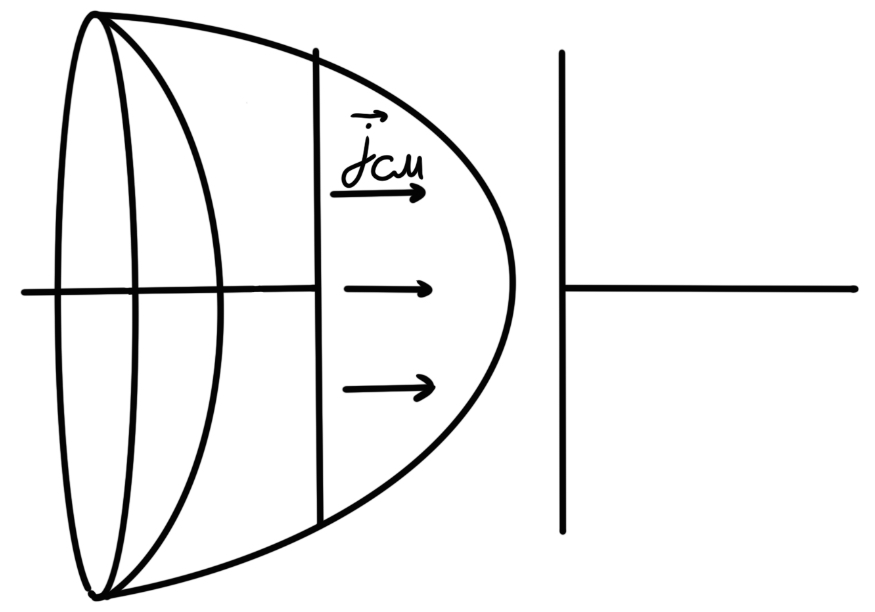
\includegraphics[width=\textwidth]{im/88.png}% Ваше изображение
\end{minipage}%
\hfill
\begin{minipage}[c]{0.6\textwidth} % Правая часть: текст
\[\underset{\delta\mathbb{S} }{\oint} \vec{H}d\vec{S}=\frac{4\pi}{c}\underset{\mathbb{S}}{\iint} \vec{j}d\vec{S} \]
\end{minipage}

\begin{minipage}[c]{0.3\textwidth} % Левая часть: изображение
    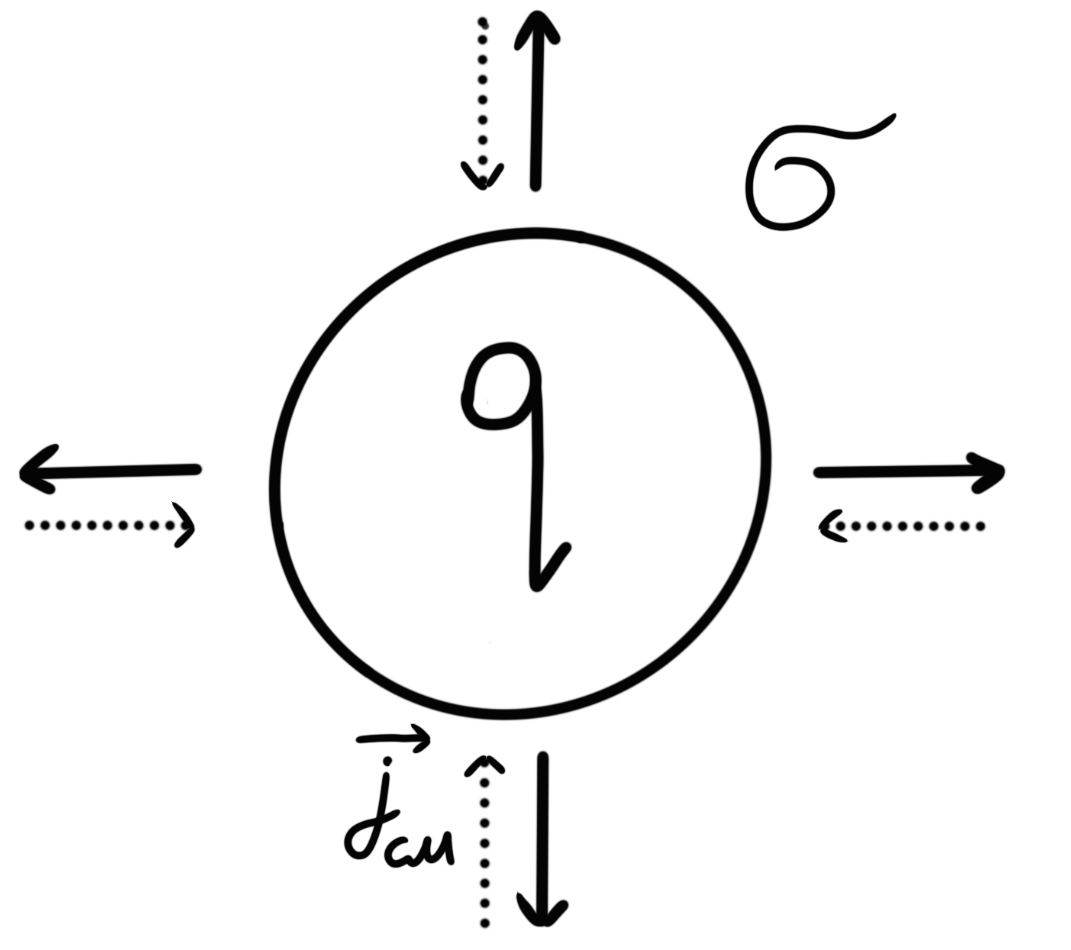
\includegraphics[width=\textwidth]{im/89.png}% Ваше изображение
\end{minipage}%
\hfill
\begin{minipage}[c]{0.6\textwidth} % Правая часть: текст
\[
\begin{aligned}
&\text{Максимальная релаксация:} \\
&\text{магнитное поле всюду ноль отсюда}:\\
&\mathrm{rot}\vec{H}=0 \text{ , отсюда } \vec{j}=0 \\
&\text{, а это не верно, значит уравнение не полное}
\end{aligned}
\]
\end{minipage}

Дополнение:

\[
\mathrm{rot}\vec{H}=\frac{4\pi}{c}\left( \vec{j}+\vec{j}_{\text{см}} \right)\Rightarrow \mathrm{div}\vec{j}=-\mathrm{div}\vec{j_{\text{см}}}=-\frac{\partial\rho}{\partial t}=-\frac{1}{4\pi}\mathrm{div} \frac{\partial \vec{D}}{\partial t}        
\]

Если принять \( \vec{j_{\text{см}}}=\frac{1}{4\pi}\frac{\partial \vec{D}}{\partial t}     \) , то получим дополненое уравнение Максвелла:

\[
\boxed{\mathrm{rot}\vec{B}=\frac{4\pi}{c}\vec{j}+\frac{1}{c} \frac{\partial\vec{D}}{\partial t}    }
\]

\begin{gather*}
    \vec{D}=\vec{E}+4\pi\vec{P} \\
    \frac{\partial \vec{D}}{\partial t}= \frac{\partial \vec{E}}{\partial t} +4\pi \frac{\partial \vec{P}}{\partial t}  
\end{gather*}

Уравнение Максвелла:

\[
\begin{aligned}
    \begin{cases}
        \mathrm{div}\vec{D}=4\pi\rho \\
        \mathrm{rot}\vec{E}=-\frac{1}{c} \frac{\partial\vec{B}}{\partial t} \\
        \mathrm{div}\vec{B}=0 \\
        \mathrm{rot}\vec{H}=\frac{4\pi}{c}\vec{j}+\frac{1}{c} \frac{\partial D}{\partial t}      
    \end{cases}
    \text{ }
    \begin{array}{ll}
        \oiint \vec{B}d\vec{S}=0 \\
        \oint\vec{H}d\vec{l}=\frac{4\pi}{c}I+\frac{1}{c} \frac{\partial}{\partial t}\iint \vec{D}d\vec{S} \\
        \text{где } I=\underset{\mathbb{S}}{\iint}\vec{j}d\vec{S} 
    \end{array}
\end{aligned}
\]

Мат. уравнения:

\[
\vec{D}=\varepsilon\vec{E} \qquad \vec{B}=\mu\vec{H}
\]

Закон сохранения зарядов уже входит в уравния Максвелла.

\section{Квазистационарные электромагнитные поля. Уравнение диффузии для
магнитного поля. Скин-эффект.}

\subsection*{Скин-эффект}



\section{Энергия магнитного поля системы контуров с током. Коэффициенты само-
и взаимоиндукции. Симметричность матрицы коэффициентов Lik.}

\subsection*{Энергия магнитного поля системы контуров с током}

\textit{Для одного контура:}

Ток I идет по замкнутому контуру.

\begin{gather*}
    \varepsilon=-\frac{1}{c}\frac{d\Phi}{dt}; \qquad \varepsilon_{\text{ист.}}=\frac{1}{c}\frac{d\Phi}{dt} \\
    dW=I\varepsilon_{\text{ист}}dt=I \frac{1}{c}\frac{d\Phi}{dt}=\frac{1}{c}Id\Phi     
\end{gather*}

\textit{Для нескольких контуров:}

\begin{minipage}[c]{0.4\textwidth} % Левая часть: изображение
    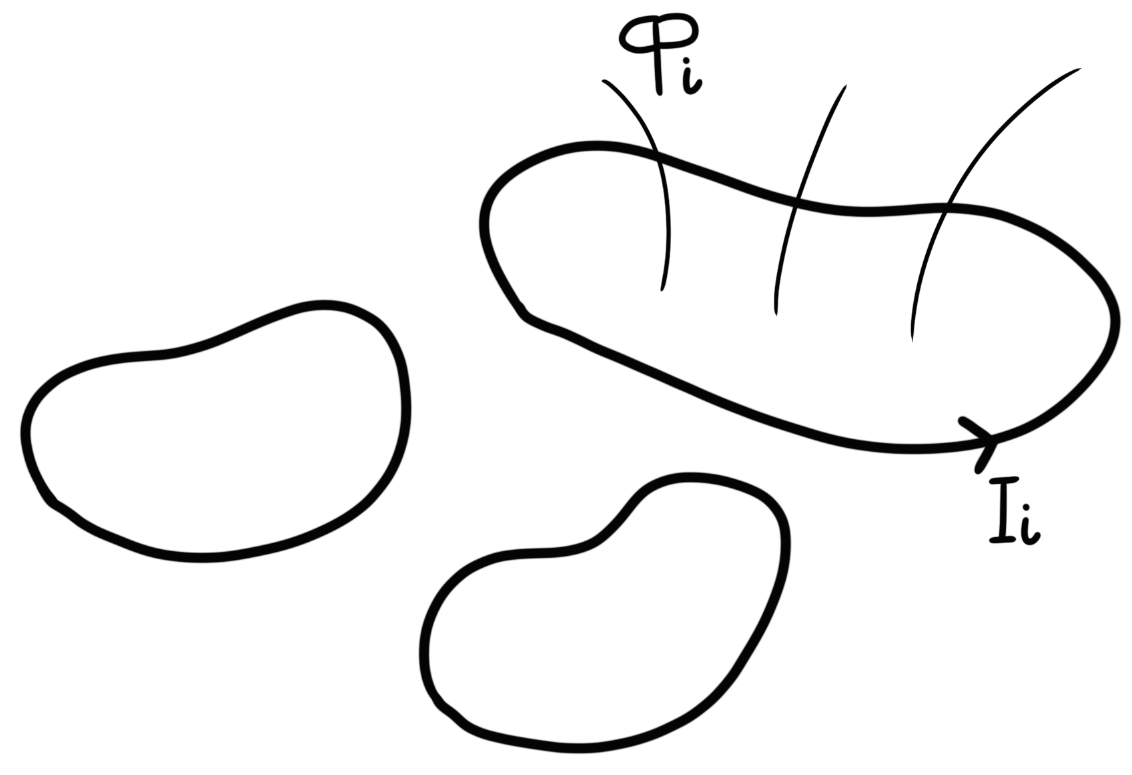
\includegraphics[width=\textwidth]{im/93.png}% Ваше изображение
\end{minipage}%
\hfill
\begin{minipage}[c]{0.6\textwidth} % Правая часть: текст
    \begin{gather*}
        \text{При } I_i=0 \quad W=0 \\
        dW=\frac{1}{c}\sum_{i}I_id\Phi_i 
    \end{gather*}
\end{minipage}

В случае линейной среды:

\[
\tilde{I}_i=\alpha I_i \text{ , где }0\leqslant \alpha\leqslant 1 \Rightarrow \tilde{\Phi}_i=\alpha \Phi_i \text{ и } d\tilde{\Phi}_i=\Phi_i d\alpha
\]

\[
W=\frac{1}{c} \sum_{i}\tilde{I}_id\tilde{\Phi}_i=\frac{1}{c}\sum \int \alpha I_i \Phi_i d\alpha=\sum_{i}\frac{1}{c}\Phi_i I_i \int_{0}^1\alpha d\alpha=\sum \frac{1}{2c}\Phi_i I_i    
\]

В случае линейной среды: \( \boxed{W=\frac{1}{2c}\sum_{i}\Phi_iI_i } \) 

В случае нелинейной среды: \( \boxed{dW=\frac{1}{c}\sum_{i}I_id\Phi_i } \) 

Энергия магнитного поля через: \( \vec{A} \text{ и } \vec{j} \) 

\[
\text{Поток: } \Phi=\underset{\mathbb{S}}{\iint}\vec{B}d\vec{S}=\underset{\mathbb{S}}{\iint}\mathrm{rot}\vec{A}d\vec{S}=\underset{\delta\mathbb{S}}{\oint}\vec{A}d\vec{l} 
\]

Тогда: \( \frac{1}{2c}\sum_{i}\underset{\mathbb{L}}{\oint}I_i \vec{A}d\vec{l}  \) при переходе к распределенным токам: 

\( Id\vec{l}\rightarrow\vec{j}dV \):

\[
\boxed{W=\frac{1}{2c}\iiint \vec{A}\vec{j}dV }
\]

Аналогично для нелинейной среды: 

\[
\boxed{\delta W=\frac{1}{c}\iiint \vec{j}\delta \vec{A} dV }
\]

\subsection*{Коэффициенты само-
и взаимоиндукции и Симметричность матрицы коэффициентов Lik.}

\[
    \begin{pmatrix}
        \Phi_1 \\
        \Phi_2 \\
        \vdots \\
        \Phi_i \\
        \vdots
        \end{pmatrix}
        =
        \renewcommand{\arraystretch}{1.8} % Увеличивает вертикальные интервалы в матрице
        \setlength{\arraycolsep}{1.2em}   % Увеличивает горизонтальные интервалы между столбцами
        \frac{1}{c} 
        \begin{pmatrix}
           &   &   \\
           & \overset{\wedge}{L} &   \\
           &   &  
        \end{pmatrix}
        \quad
        \renewcommand{\arraystretch}{1.} 
        \setlength{\arraycolsep}{1.2em}   
        \begin{pmatrix}
        I_1 \\
        I_2 \\
        \vdots \\
        I_i \\
        \vdots
        \end{pmatrix}
        \quad
\]

Где \(\overset{\wedge}{L}\) - матрица индуктивных коэффициентов

\[
\Phi_i= \frac{L_{ij}I_i}{c} \quad L_{ij}\text{- коэф. самоиндукции} 
\]

Докажем, что \(  L_{ij}=L_{ji} \):

\begin{gather*}
    \left[ W = \frac{1}{2c}I_i\Phi_i, \; dW = \frac{1}{c}I_i d\Phi_i \right] 
    \Rightarrow \frac{1}{2}d(I_i\Phi_i) = I_i d\Phi_i, \\
    \frac{1}{2}\Phi_i dI_i + \frac{1}{2}I_i d\Phi_i = I_i d\Phi_i 
    \Rightarrow \Phi_i dI_i = I_i d\Phi_i, \\
    \frac{1}{c}L_{ij}I_idI_i=I_iL_{ji}\frac{1}{c}
    \Rightarrow (L_{ij}-L_{ji})I_jdI_i=0 \Rightarrow L_{ij}=L_{ji} \quad \blacksquare 
\end{gather*}

\[
W=\frac{1}{2c^2}L_{ij}I_iI_j 
\]

Для самоиндукции:

\[
W=\frac{1}{2c^2}LI^2 
\]

\end{document}
